%
\chapter{Bolometry at W7-X}\label{chap:bolometry}%
%
    The word bolometer is derived from the greek \textgreek{βολή} (\textit{boli}), meaning "beam" or "cast", and \textgreek{μετερ} (\textit{meter}), "to measure". Therefore, the purpose of a bolometer can be noted as \textit{to measure beams of light}. Its principle was invented by american astronomer \textit{Samuel Pierpont Langley}\footnote[1]{Samuel Pierpont Langley * Aug. 22, 1834 \textdagger~Feb. 27, 1906} in 1878 and was later used for infrared measurements at the Allegheny Observatory\cite{Langley1880,Langley1881}. Their results were involved in first calculations made by \textit{Svante Arrhenius}\footnote[2]{Svante August Arrhenius *~Feb. 19, 1859 \textdagger~Oct. 2, 1927} in 1896 regarding the greenhouse effect\cite{Arrhenius1896}.\\%
%
    \newline%
    A bolometer consist of an absorber, which is (thermally) linked to a reservoir with ideally constant properties. Incident energy, either through photons, impinging particles or even non-observable dark matter results in a change of state, i.e. temperature, of the absorber in relation to the reservoir. In proportion to the amount of absorbed energy this difference increases, which is relaxed into the reservoir at a speed defined by an intrinsic time constant, specific capacity and conductance between absorber and reservoir. In the case of thermal detectors the absorber works as a resistive thermometer, whose cooling time, heat capacity and thermal conductance can be used to calculate incident power from a change in temperature.\\%
    Bolometers are widely used today in both industry and different fields of science. At ultra-low temperatures, e.g. below \SI{10}{\kelvin} or less, they can be used as particle detectors, or in the case of the \tilt{Herschel Space Observatory}\cite{Gildemeister1999} and \tilt{Stratospheric Observatory for Infrared Astronomy} (SOFIA), as detectors for cosmic radiation.\cite{Huebers2000} Thermal cameras consist of a large array of \tilt{microbolometers} that acquire radiation in the spectral infrared range\cite{Kumar2003}.\\%
    \,\newline%
    The following chapter will briefly introduce the bolometer diagnostic in plasma fusion devices and specifically characterize the one implemented at the stellarator Wendelstein 7-X.%
%
    \section{Overview}\label{sec:concept}%
%
        % Overview.
        The purpose of bolometers in fusion devices is to measure the spatial and temporal evolution of the irradiated power from the plasma within their field of view and sensitive spectral range. Depending on the type and construction, this can be, but not limited to, from infrared to soft X-ray. Additionally, the diagnostic has to conform to high operational demands governed by the circumstances in such machines\cite{Giannone2002}. The performance of bolometers in plasma fusion devices has to be unaffected by large changes in ambient temperature, as well as high thermal loads for extended durations, e.g. as is the case at Wendelstein 7-X. They need to withstand neutron radiation and consequently a radioactive contamination, while being insensitive to large electromagnetic fields and pressure perturbations. The most crucial requirement to a bolometer is however the consistency and reliability of its measurements due to very limited access to and maintenance of the diagnostic after it has been installed in a fusion device. As we will see later in \autoref{sec:geomimpact}, this especially holds true for the geometry of the diagnostic. Because of the application of methods of inversion on the bolometric measurements in order to find the local radiation distribution, the line of sight geometry has to be as accurate as possible. Perturbations by thermal and mechanical stresses exerted on the machine during evacuation and cooling need to be negligible. Furthermore, in the case of the bolometer at W7-X, an \textit{in-situ} calibration of the above-mentioned parameters, which provides information about the current state of the diagnostic, needs to be carried out reliably. Finally, the small measurement signals need to be transferred outside the vacuum vessel for a long distance to the data acquisition hardware in environments with strong interference and background noise.\\%
        The following chapter will present the bolometer diagnostic that has been implemented and established at W7-X, which the enclosed results of this work will rest upon. The conception, implementation and deployment of a \textit{\textbf{real-time radiation system}} that is designed to provide information about the radiation power loss for plasma feedback-control purposes is a key issue of this thesis. Starting with \cref{sec:w7xbolometer}, the necessary theoretical and experimental background will be provided in order to properly introduce the bolometer as such, as well as the radiation feedback system later on in \cref{chap:realtimefeedback}.%

        \subsection*{Detector Species}\label{subsec:detectoradvant}%
%
            % Detector species.
            Over the past forty years\cite{Husan1975}, bolometers have been widely adapted in plasma fusion devices. The most prevalent concepts are the metal resistor bolometer, \tilt{absolute extreme ultraviolet} (AXUV) photo diode bolometer and \tilt{infrared imaging video bolometer} (IRVB), while there exist other designs like ferroelectric\cite{Maio1997} or semiconductor\cite{Iborra1993} bolometers, which are not applied in fusion devices.%
%
            \paragraph{Metal Resistor Bolometer}%

                % Metal resistor bolometer.
                The metal resistor bolometer is the most common concept found in plasma fusion devices. Modern designs consist of highly sensitive thin metal film absorbers, residing on electrically non-conductive thermal transmission layers that are connected to a metal resistor. Additional to the thin metal film, a nanometer thick carbon coat can be applied to enhance the spectral responsiveness of the absorber in the infrared range\cite{Zhang2010}. They generally feature operational reliability, resilience against the hostile environments found in fusion devices and low sensitivity for perturbations in parameters like pressure or ambient temperature\cite{Mueller1984}.%
%
            \paragraph{Absolute Extreme Ultraviolet Bolometer}%

                % AXUV bolometer.
                The absolute extreme ultraviolet bolometer uses p-n junction photodiodes with a sensitive spectral range from ultraviolet to X-ray radiation, very fast temporal responsiveness and insensitivity to impinging neutral particles as detectors.\cite{Furno1999,Degeling2004} While being comparatively cheap and easy to use, their working principle of inner photoelectric effect limits them to a specific spectral range for acquisition, e.g. $h\cdot\nu>E$\footnote[1]{photon energy: $h$ \textit{Planck} constant, $\nu$ frequency, $E$ energy}$^{,}$\footnote[2]{Max Karl Ernst Ludwig Planck *~April 23, 1858, \textdagger~Oct. 4 1947}. Due to their nonlinear frequency response and degradation in fusion environments they are not applicable for absolute radiation power measurements. Additionally, photodiodes degrade over time, especially due to the incoming neutron flux from D-T processes and strong $\gamma$ radiation. Therefore, AXUV bolometers are more likely to be used complimentary to other bolometric diagnostics in order to resolve fast events and complement commonly resistive systems.\cite{Bernert2014}
%
            \paragraph{Infrared Imaging Video Bolometer}%
%
                % IRV bolometer.
                Infrared imaging video bolometers or segmented mask infrared imaging bolometer (\tilt{SIB}) measure radiation with a single, large metal foil behind a slit aperture or pinhole. The change in foil temperature due to incident radiation is measured from the carbon coated backside with an infrared camera, between which an IR transmitting vacuum window is placed to eliminate cooling through convection. In case of the SIB, the thin metal film is clamped between two masks, in most cases made out of copper as a heat sink, exposing an array of pixels on both sides. Properties and performance of the bolometer therefore are governed by pixel size, material thicknesses and mask attributes. The IRVB does not use masks on either side and thus has to rely on a delicate calibration for the thermal diffusion model of the metal film, which in turn rewards with an increase of detector area of ca. 40\% and the removal of shadowing from mask to pixel\cite{Peterson2000,Peterson2016}. The local power deposition is derived by solving the two-dimensional heat transport equation on the thin foil. At the Large Helical Device (\tilt{LHD}) a reliable calibration method has been established\cite{Peterson2003_1,Pandya2014}. Like the metal resistor detector, it can be used in demanding conditions such as plasma fusion devices, while having good spatial and temporal resolution. Drawbacks include the complicated diffusion modelling, the spectral sensitivity and the dependency between responsiveness and thickness, balancing the range of photons energies than can be absorbed and time resolution\cite{Peterson2003_2}.\\%
%
        In the following chapter the thin metal film resistor bolometer, as implemented at the stellarator Wendelstein 7-X will be discussed. Their kind is the most promising candidate for long term usage at future deutereum-tritium plasma fusion reactors, as they potentially meet all projected operation requirements\cite{Meister2008}, although IRVB bolometer types have been discussed for future fusion devices such as ITER\footnote[1]{ITER: International Thermonuclear Experimental Reactor} as well.%

    \section{W7-X Bolometer Diagnostic}\label{sec:w7xbolometer}%
%
        % Core bolometry at W7-X.
        The bolometer diagnostic at the stellarator W7-X measures the irradiated power from the plasma. It provides the total radiated power loss for global power balance studies and information about transport. In terms of plasma diagnostics, one important property under investigation is the radiation power loss. The overall radiation distribution and transport, mainly through impurities but also neutral particles, as well as the global power balance are of large importance.\\%
        The metal resistive bolometer detectors at W7-X consist of thin metal film absorbers that are thermally connected to a resistor. Incident power by radiation or particles heats up the absorber and therefore the resistor, which in turn leads to an increase in resistance. Measuring the change in resistance, combined with knowledge about the thermal properties of the sensor, yields the absorbed power of the detector.\\%
        In order to provide spatially resolved radiation distributions from the individual line integrated measurements of each absorber an array of detectors that view the plasma through a pinhole in a camera is needed. This introduces the challenge to balance good spatial resolution, i.e.small viewing angles and narrow lines of sight, with high signal-to-noise ratios and large temperature changes in the absorber. A possible way to measure small resistance changes with high precision is the \textit{Wheatstone bridge}, where a slightly asymmetric electrical circuit of resistors experiences imbalances due to temperature change\cite{Horowitz1989}. Each bolometer detector at W7-X is connected in groups of two by a Wheatstone bridge, with two ideally symmetric reference absorbers and resistances also located inside the circuit. Setups like this have also been applied at tokamak fusion plasma experiments in the past\cite{Mast1991}.\\% 
        The detectors of the bolometer at W7-X are intrinsically very sensitive to thermal interference and non-absorbed microwave stray radiation\cite{Zhang2010}. Considerations regarding the construction and diagnostic placement were made to avoid overestimation regarding the calculation of the irradiated power from the plasma. Further requirements for the detectors are sufficient time resolution and resistance against deterioration over long term exposition inside the vessel, since later adjustments during operational campaigns are not possible. Furthermore, calibrations can only be done prior to construction and, once assembled, inside the device, so that only an in-situ procedure gives access to any detector parameters needed for calculations.\\%
        \,\\%
%
        This section is devoted to introducing the measurement principle and design of the bolometer at W7-X. One will thoroughly present the implemented construction of the device and the resulting features in regard to the experimental environment. To start, the requirements imposed by the fusion experiments itself, which in turn lead to decisions regarding the design will be discussed.%
%
        \subsection{Requirements}\label{sec:requirements}%
%
            % Requirements.
            Wendelstein 7-X is designed to be capable of a steady-state operation at \SI{10}{\mega\watt} of \SI{140}{\giga\hertz} microwave electron cyclotron resonance heating for at least \SI{30}{\minute}. The total non-absorbed microwave power will be limited to \SI{1}{\mega\watt}, which equals an ECRH stray radiation flux density of \SI{90}{\kilo\watt\per\square\meter} on plasma facing components. Higher values are expected close to the heating beam launchers and about a factor of ten less in places opposite to the ECRH launching antennas\cite{Hathiramani2013}. This microwave stray radiation will impact on plasma facing components and diagnostics after multiple path reflections inside the vessel. Therefore, diagnostics facing the plasma which are susceptible to the microwave disturbance like the bolometer need special considerations in design\cite{Zhang2010}. A potential bolometer detector and data acquisition (DAQ) system at W7-X are also expected to be able to continuously measure the radiation power coming from the plasma for \SI{30}{\minute} without degradation. Due to restrictions on in-vessel work, the diagnostic ideally requires no repetitive or extensive servicing, i.e. calibration, repair or exchange of aging components.\\%
            The radiative power loss from the plasma and non-absorbed microwave radiation are expected to average to multiple \SI{10}{\kilo\watt\per\square\meter} thermal load on plasma facing structures. Components closer to emitting microwave antennas or with higher absorption coefficients face additional challenges\cite{Koenig2010,Burhenn2011}. Due to its design the metal resistor bolometer is especially susceptible to stray microwave radiation and thermal perturbations. During machine preparation components are conditioned by "\tilt{baking}" them for a long duration with a radio frequency discharge at around \SI{150}{\celsius}. A thermal siphon has to be attached to the detector to provide a large enough mass and short cooling time, which prevents the absorber from damaging through thermal loads. Finally, possible deuterium plasma operation imposes the question about neutron resilience and lifecycle of the detector.\\%
            The bolometers lines of sight have to be carefully planned in order to achieve the best possible spatial resolution while covering as much poloidal cross-section as possible at their respective toroidal position. Due to the intrinsic design of W7-X, the insertion port for the diagnostic is cylindrical shaped, thus limiting the geometry of a possible bolometer camera. Radiation from the plasma should be absorbed evenly across a wide spectral range, e.g. visible light to soft X-ray, so an absolutely calibrated power measurement is possible.%
%
        \subsection{Construction}\label{subsec:construction}%

            % Construction.
            The bolometer diagnostic at W7-X consists of a two-camera system of thin metal film resistive detectors. The schematic of a single detector can be seen in \cref{fig:detector_me}. The 3.8$\times$\SI{1.3}{\milli\meter}, \SI{5}{\milli\meter\squared} absorber consists of a \mbox{\SI{5}{\micro\meter}} thick gold film, enclosed by a \mbox{\SI{0.6}{\milli\meter}} thick Si front plate frame, which resides on a \mbox{\SI{5}{\micro\meter}} Si$_{3}$N$_{4}$ layer. A \mbox{\SI{150}{\nano\meter}} aluminium layer covers both gold detector and silicone frame. The detector area is covered by a thin \mbox{\SI{50}{\nano\meter}} carbon coat. On the silicon-nitrate substrate, two \mbox{\SI{1}{\kilo\ohm}} Pt meanders from the Wheatstone brigdge connect to the electrical circuit for data acquisition. Besides this \textit{main} absorber design there also exist \textit{secondary}, beryllium or aluminium covered absorbers that can be used for the focused analysis of high impurity radiation in the soft X-ray range due to their respective spectral properties.\\%
%
            \begin{figure}[t]%
                \centering%
                \includegraphics[width=0.7\textwidth]{%
                    content/figures/chapter1/detector_me}%
                \caption{%
                    Detector schematic. Diagram of a single blackened detector foil with frame, substrate and meander. Layer dimensions are noted, however not pictured to scale}\label{fig:detector_me}%
            \end{figure}%
%
            Behind the silicon frame, four of the eight total absorbers per detector chip are hidden, so that they are shut off from radiation and therefore should not experience a change in temperature. This chip of absorbers, electrical circuit and meander is placed between the silicon frame and an aluminium backplate, which resides on a ground plate with pin connectors for data acquisition. The top to bottom, i.e. from plasma side to pins, assembly schematic can be seen in \cref{fig:assembly}. Two of each absorber type, measurement and reference are connected in a Wheatstone bridge on the chip like \cref{fig:chip}. The non-exposed reference absorbers can be seen on the right half of the chip in \cref{fig:assembly}, where the solid part of the front plate is covering them in contrast to the recesses on the left. Small drill holes in the front plate close to the reference foils are dedicated to equilibrating ambient pressure changes for both absorbers, while still providing full coverage from radiation. The exposed measurement and closed-off reference absorber form the Wheatstone bridge for data acquisition. The schematic of an electrical circuit for a Wheatstone bridge as constructed by reference and measurement absorbers can be seen in \cref{fig:wheatstone}. Further details on its physical measurement principle will be discussed in \cref{subsec:bolometerequations} when introducing the bolometer equations.\\%
%
            \begin{figure}[t]%
                \centering%
                \begin{subfigure}{0.375\textwidth}%
                    \centering%
                    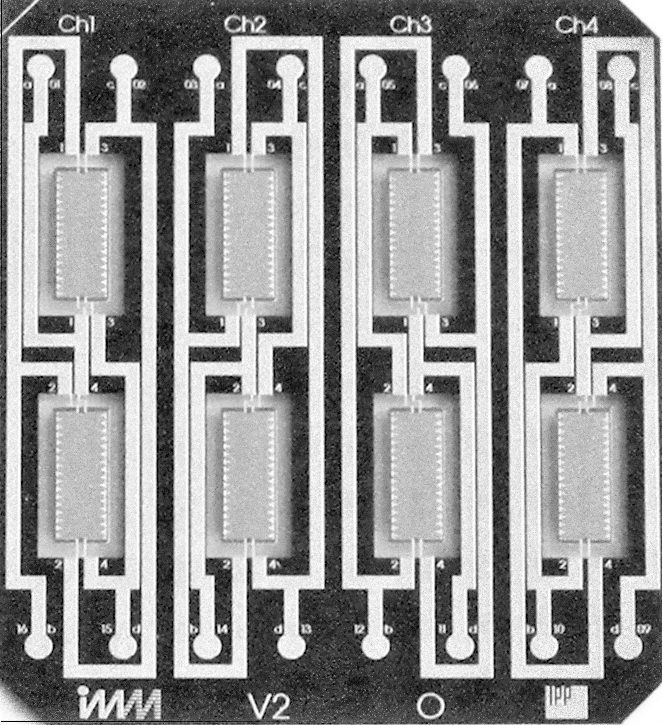
\includegraphics[width=\textwidth]{%
                        content/figures/chapter1/detector_backside_bw.png}%
                    \vspace*{0.25cm}%
                    \caption{Detector chip}\label{fig:chip}%
                \end{subfigure}%
                \hspace*{1.0cm}%\hfill%
                \begin{subfigure}{0.33\textwidth}%
                    \centering%
                    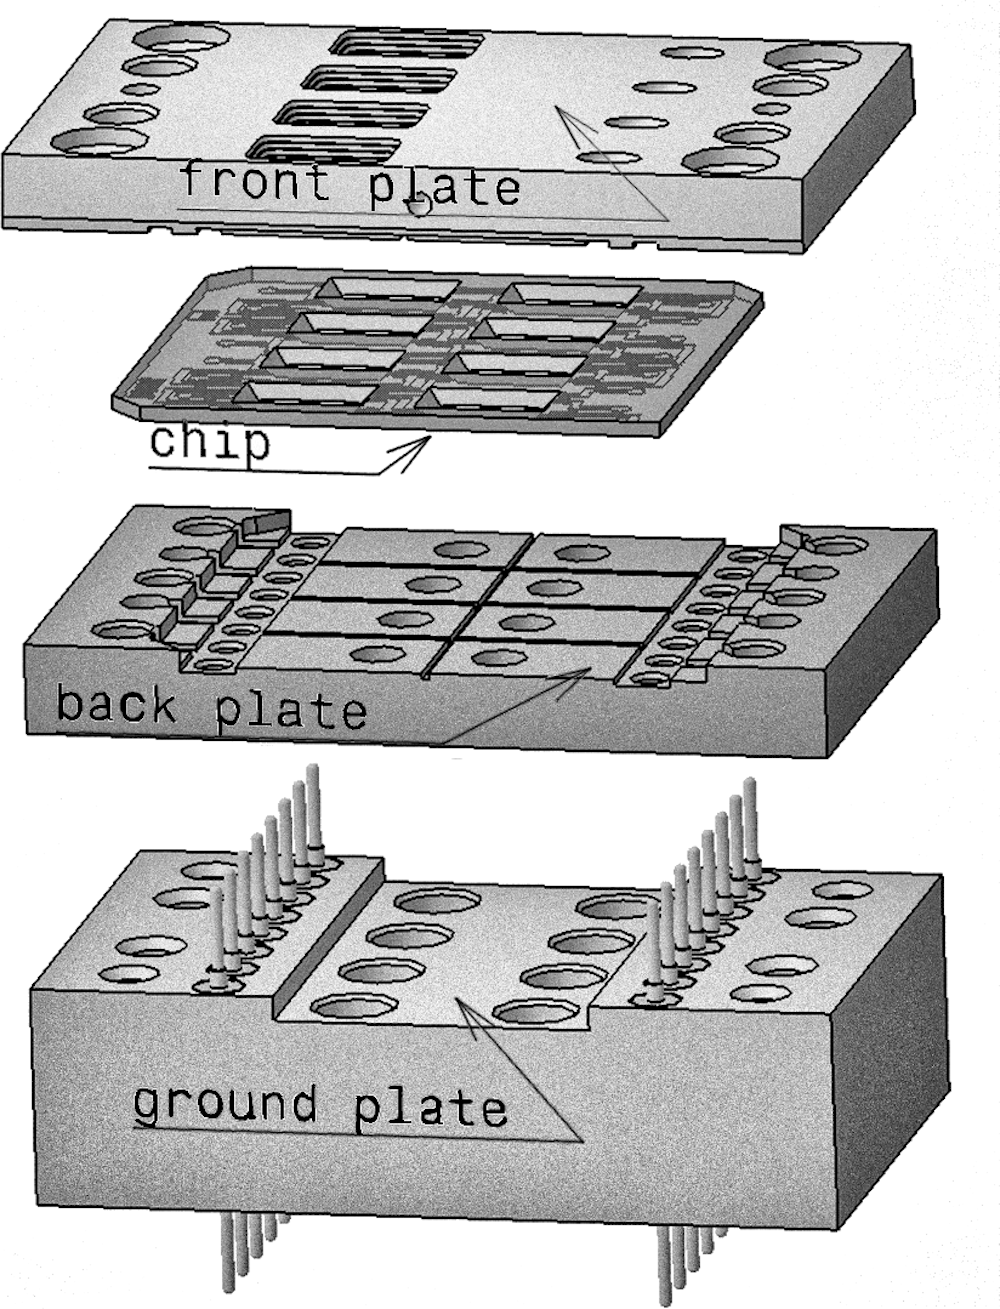
\includegraphics[width=\textwidth]{%
                        content/figures/chapter1/bolometer_assembly_daz_bw}%
                    \caption{Bolometer head}\label{fig:assembly}%
                \end{subfigure}%
                \caption{(Left) Detector chip backside with four reference and measurement absorbers each connected in Wheatstone bridges as pairs. (Right) Bolometer group head assembly from plasma side (top) to cable connection pins (bottom).}\label{fig:wheatstone_assembly}%
            \end{figure}%
%
            The bolometer system at W7-X incorporates two cameras that are each made up out of multiple detector arrays that consist of 32 measurement and reference absorbers. The detector arrays are located behind a graphite camera front plate with pinholes through which each views the plasma individually. Between the two pinholes in each camera front plate and the detector arrays located behind there is a rotary shutter that is capable of blocking any radiation entering the housing. The detector holder, camera housing and aperture are all cooled via the central water cooling system of W7-X, which is coupled to a several hundred cubic meter large reservoir. Temperature changes of the camera array are monitored by a Pt100 resistive thermometer integrated into the back. A full camera head assembly with two detector arrays inside can be seen in \cref{fig:component_3D}. The individual arrays are located as close to each other as possible so that their resulting lines of sight view approximately the same plasma volume. The absorber chips with their assembly in \cref{fig:assembly} are collected in a group head with four channels per unit each. These group heads are angled individually towards the pinhole inside the camera array in a fan-shape to achieve the best possible line of sight coverage of the plasma at small viewing angles.\\%
%
            \begin{figure}[t]%
                \centering%
                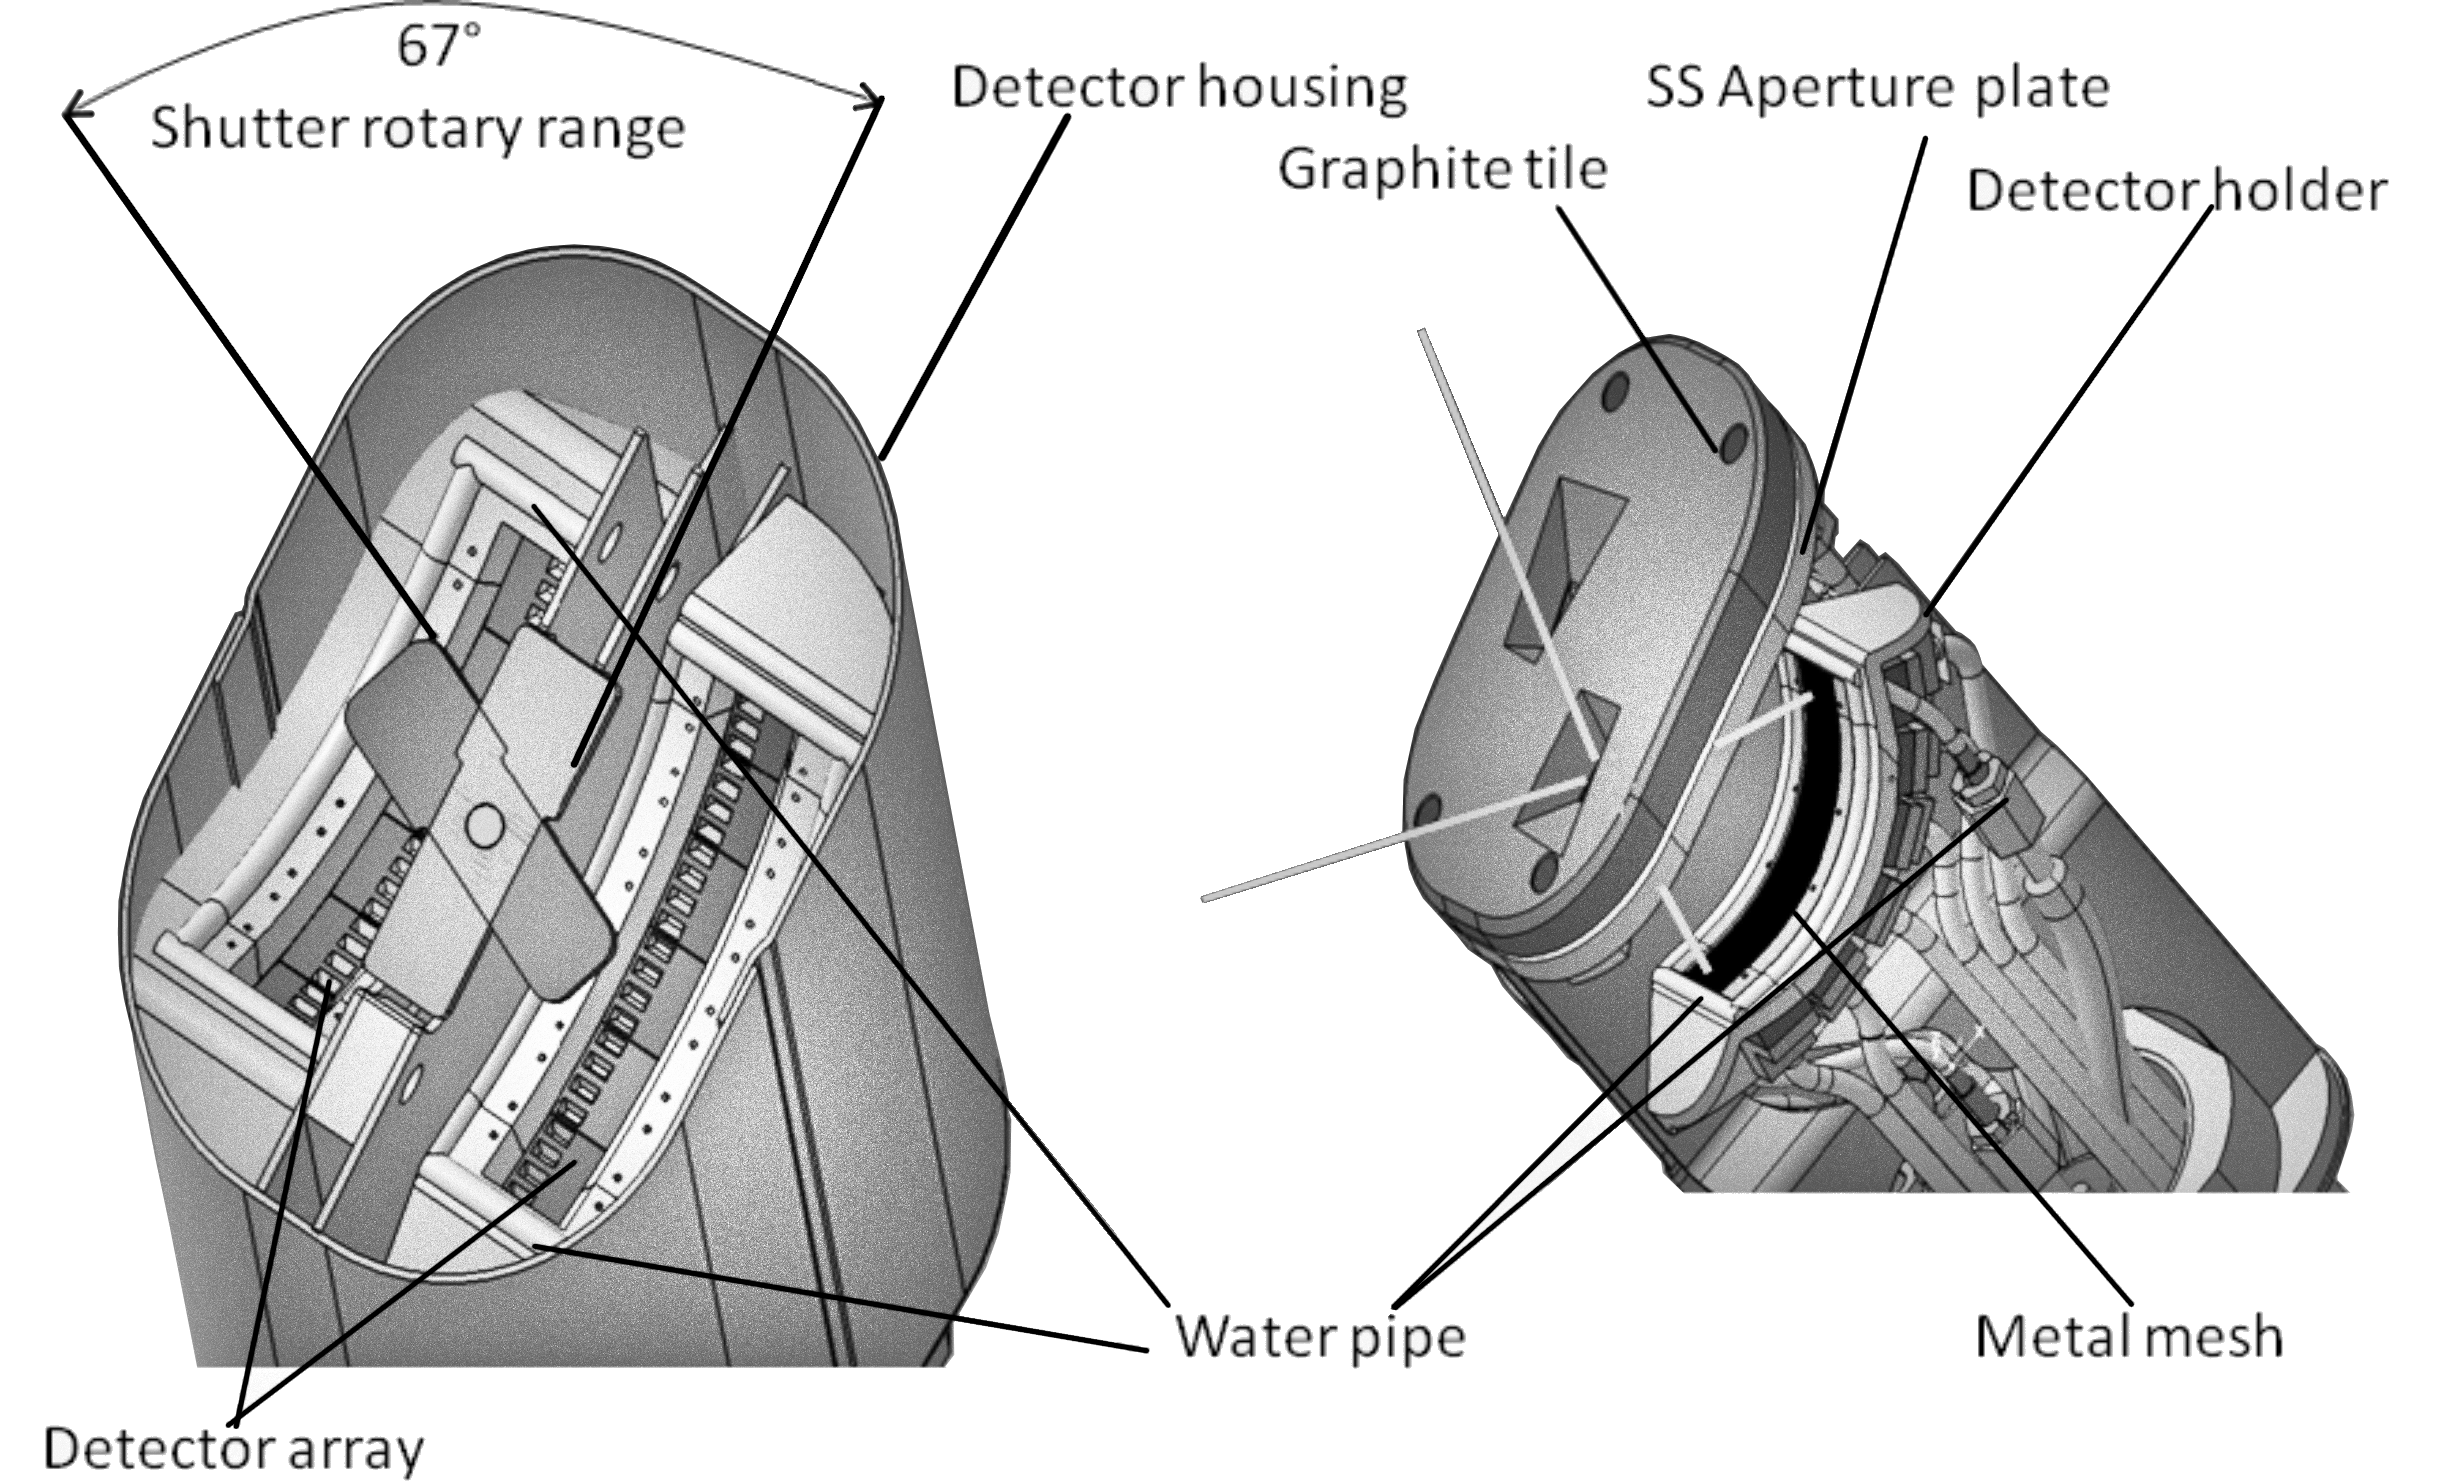
\includegraphics[width=0.7\textwidth]{%
                    content/figures/chapter1/component_3d_bw_alpha}%
                \caption{%
                    Overview of one (vertical bolometer) camera head. (Left) Two subdetector arrays mounted on two water cooled detector holders, separated with an optic baffle, behind a rotating shutter inside the ellipsoidal camera head at the front of the diagnostic port. (Right) Graphite tile cap in front of the stainless steel aperture plate as thermal protection with indicated line of sight cone, wire mesh microwave protection and backplate connectors.}\label{fig:component_3D}%
            \end{figure}%
%
            The detector system is connected via shielded ultra-high vacuum (UHV) proof, low resistance, low impedance, \mbox{\SI{40}{\meter}} long cables, which are terminated in ten pole LEMO® connectors on both sides, to the data acquisition chassis outside the fusion device. Four master base printed circuit boards (PCB) connect to 32 individual data acquisition (DAQ) cards each, which contain the analog-to-digital converter (ADC) AD7730 from \mbox{National Instruments\textsuperscript{\textregistered,}}\footnote[1]{National Instruments (NI), NASDAQ: NATI; Austin, TX. USA, founded 1976}. Every individual measurement-reference absorber pair is connected via the cables to on of the DAQ cards. The four master PCBs are connected via ribbon cables with individual pins for each DAQ card to a \mbox{NI\textsuperscript{\textregistered} 7813R}. The entire 128 channel system is controlled via a \mbox{LabVIEW\textsuperscript{\textregistered,}}\footnote[2]{Laboratory Virtual Instrumentation Engineering Workbench, National Instruments 1986} software program, consisting of both controls for the analog-to-digital converters (ADC), as well as graphical user interface for diagnostics and debugging. Data of an ongoing measurement is stored in volatile random access memory (RAM). Before it is uploaded via an Ethernet link to the central Wendelstein 7-X archive data vault for redundancy, an individual local copy is stored on the onboard hard drive disk (HDD).%
%
        \subsection{Line of Sight Geometry}\label{subsec:losgeometry}
%
            % Line-of-sight geometry.
            To achieve the best possible results when evaluating the line of sight integrated data from each detector and calculating the radiated power distribution, the camera geometry has to provide good coverage of the plasma cross-section. The two cameras are located at slightly offset toroidal positions around \SI{108}{\degree} toroidally, in the \textit{triangular} plane of W7-X. One camera head is located on the outer side of the vessel, watching the plasma horizontally, while the other is positioned below, viewing vertically into the vessel. Both devices are angled in toroidal direction due to the shape and orientation of the vessel diagnostic mounting. Their identical intrinsic tilt is, according to the structural design, \SI{68.75}{\degree}, which gives the detector lines of sight a toroidal extension of $\approx\SI{5}{\degree}$. The center-center, i.e. center of detector traced through the center of the aperture, line of sight distribution for both camera heads can be seen in \cref{fig:los_vessel}.\\%
%
            \begin{figure}[t]%
                \centering%
                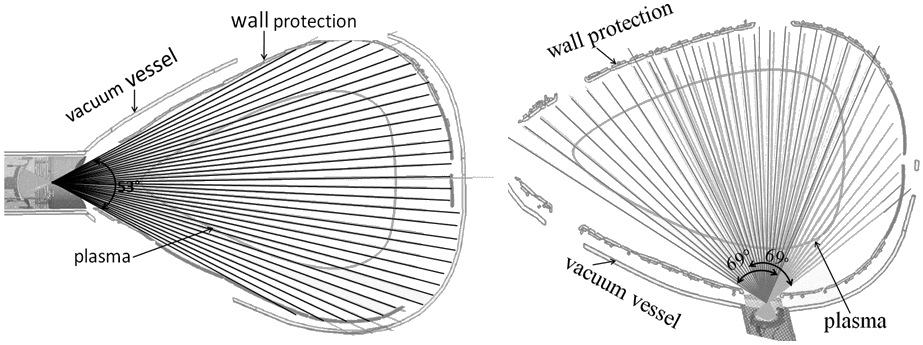
\includegraphics[width=0.9\textwidth]{%
                    content/figures/chapter1/HTPD_BW}%
                \caption{Lines of sight of (left) horizontal bolometer camera, consisting of 32 individual detectors, and (right) vertical bolometer possessing two subdetector arrays of 24 channels each, viewing the plasma through their own respective apertures.}\label{fig:los_vessel}%
            \end{figure}%
%
            The horizontal bolometer camera (HBC) is divided into two 32 channel subarrays, where one is designed and built as described in \cref{subsec:construction}. The same is true for the vertical bolometer camera (VBC). In the latter case, the two arrays are made up out of 32 channels each, however both have 24 standard channels like before, where their lines of sight overlap around the poloidal center of the vessel.\\%
            The HBC covers the entire vessel cross-section horizontally, which guarantees complete coverage for plasma radiation in varying magnetic configurations. The VBCs lines of sight do not cover the full scrape-off layer at the bottom of the machine, but only the magnetically confined plasma area. The intersecting lines of sight of HBC and VBC provide the possibility to perform tomographic inversion of the line-integrated measurements. For further reference one can look at \cref{chap:inversions} where such mathematical tools will be applied to the bolometer data.\\%
            Due to their relative position to the plasma, and thus different requirements for the opening angle, the aperture to detector distance varies between the cameras. The detectors of the horizontal camera are \SI{175}{\milli\meter} and of the vertical camera \SI{84}{\milli\meter} equidistantly placed behind the pinhole. Each of the detectors lines of sight are collimated through their respective pinhole. They are arranged in a shape of an arch or fan, as shown in \cref{fig:component_3D}, around the rectangular pinholes. The vertical camera features two individual apertures for the left- (VBCl) and right-facing (VBCr) subarrays to accommodate their different poloidal orientations, while the horizontal face plate only has one pinhole of 5$\times$\SI{10}{\milli\meter}, or \SI{50}{\milli\meter\squared}. The elongated side of the detectors are aligned in toroidal direction. The horizontal and vertical viewing angle of \SI{53}{\degree} and \SI{138}{\degree} for VBC and HBC - the angle between upper- (outer) and lowermost (innermost) line of sight vector.\\%
            In general, each camera head is made up out of two subsystems that are slightly offset toroidally and separated by a plate to limit the signal \textit{crosstalk} between them. The displacement is small however, so that the observed plasma volume is approximately the same for both subarrays. Furthermore, the toroidal distance between the cameras and the extent of the lines of sight in this direction are small. They are within the cameras spatial resolution around the magnetic center of the plasma of $\sim$\SI{4}{\centi\meter}.\\%
%
            \begin{figure}[t]%
                \centering%
                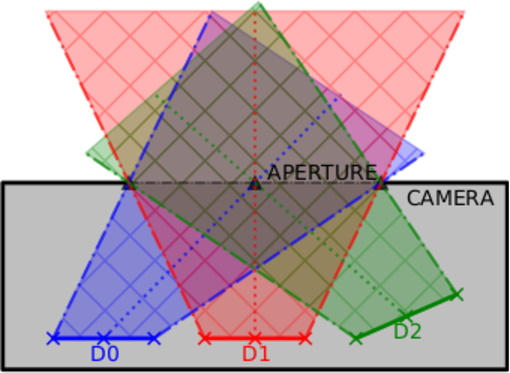
\includegraphics[width=0.4\textwidth]{%
                    content/figures/chapter1/detector_los_cones.pdf}%
                \caption{Mockup of how detectors are located in relation to their respective aperture \textbf{A} inside the camera housing \textbf{C}. \textbf{D0} and \textbf{D1} are located on the same subarray and hence in the same plane. \textbf{D2} is on another part of the camera array that is angled differently towards the pinhole.}\label{fig:loscones}%
            \end{figure}%
%
            All the chips are angled individually towards the aperture to maximize their optical transmission as shown in \cref{fig:loscones}. The lines of sight of detectors from the same subarray are qualitatively depicted by D0 and D1. They share the same plane with a small displacement in direction of the camera, i.e. along the direction of the aperture, which results in a different angle of the line of sight cones. Consequently, detectors from other subarrays, like D2, are angled differently towards the pinhole to maximize their optical transmission - as is the entire camera around the front plate aperture.\\%
%
            \begin{figure}[t]%
                \centering%
                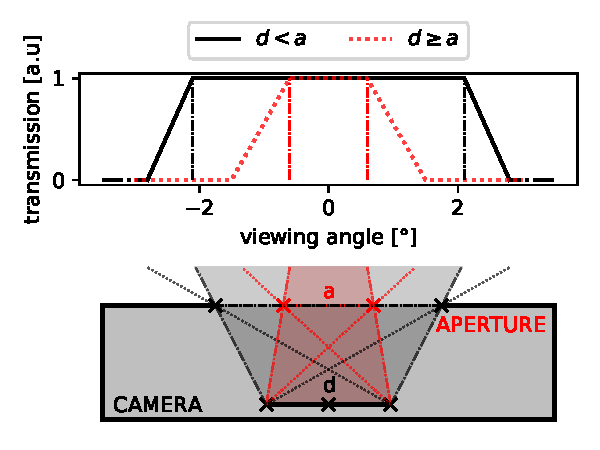
\includegraphics[width=.6\textwidth]{%
                    content/figures/chapter1/detector_los_quality.pdf}%
                \caption{Normalized arbitrary transmission functions of different size relations of aperture $a$ to detector $d$. The W7-X core bolometry is built with $d<a$.}\label{fig:transmission}%
            \end{figure}%
%
            An example of how the transmission function of a camera pinhole in relation to the projected widths of the pinhole and detector looks like can be seen in \cref{fig:transmission}. Camera, aperture and detectors shown here are not to scale and only schematically resemble the bolometers' setup. Theoretically, in a two-dimensional approximation there are two different line of sight shapes for the projection of a detector through a pinhole: trapezoidal and triangular. In the case of $d>a$ or $d\ge a$, i.e. the detector is larger or smaller than the aperture, the line of sight is of a trapezoidal shape. For the latter, the width of the \textit{cone} that is created by tracing the rectangular detector through the pinhole geometry widens the greater the distance to the aperture. The cone becomes trapezoidal. Conversely, if the pinhole is smaller than the detector the cone tapers. In relation to the distance from the pinhole, a narrowing line of sight eventually intersects with itself and therefore becomes triangular.\\%
            For all detectors of the bolometer at W7-X their respective aperture width is greater than their length, i.e. $d<a$. Hence, for this estimation we will assume the raw transmission across the line of sight cone to be unity. Investigations in \cref{sec:geomimpact} regarding the discretization of the line of sight and their respective contribution to the line integral will show for this assumption to remain valid.\\%
%
            \begin{figure}[t]%
                \centering%
                \includegraphics[width=0.5\textwidth]{%
                    content/figures/chapter1/los_angles_dist.pdf}%
                \caption{Angular relations of aperture, line of sight and detector. Angles of $\beta$ and $\alpha$ denote the angles between normals and line of sight. The distance between detector and aperture is called $d$. A lighter shade of grey indicates the partially shadowed section.}\label{fig:etendue}
            \end{figure}%
%
            \autoref{fig:transmission} also introduces a challenge for the quantitative assessment of the line of sight geometry: there exist parts of the detector that are not entirely covered by the line of sight cone where the optical transmission onto the absorber is decreased. In order to address this one needs to find the absolute light yield onto the detector through the pinhole. Assume an infinitesimal part of the detector $M$ (measurement) $\diff A_{M}$ and aperture A $\diff A_{A}$. The line of sight cone becomes a projection from $\diff A_{M}$ through $\diff A_{A}$. Let $\beta$ and $\alpha$ be the angles between the direction of the line of sight and the normals of aperture and detector, respectively. The distance between the aperture and detector is $d$. For reference, see \cref{fig:etendue}. It also more explicitly shows the partial shadowing of the detector by the projection through a pinhole. The transmission $\widetilde{K}_{M}$ can therefore be calculated using:%
%
            \begin{align}%
                \widetilde{K}_{M}=\iint_{A, M}\frac{\cos\left(\alpha\right)\cos\left(\beta\right)}{4\pi d^{2}}\,\,\diff A_{M}\diff A_{A}\,\,.\label{eq:etendue_woline}%
            \end{align}%
%
            \autoref{eq:etendue_woline} is called \textit{etendue} and is a measure for the light-yield onto the detector through the pinhole. The etendue addresses the problem of partial coverage of the absorber with the incident angles $\alpha$ and $\beta$ inside the integral. Furthermore, the previously addressed spatial resolution of the bolometer camera is defined by the width of the cone where the optical transmission or light yield is maximum. A more detailed discussion of the mathematical approach to the line of sight geometry and impact on radiation power calculations can be found in \cref{sec:geomimpact}.\\%
%
            \begin{figure}[t]%
                \centering%
                \begin{subfigure}{0.4\textwidth}%
                    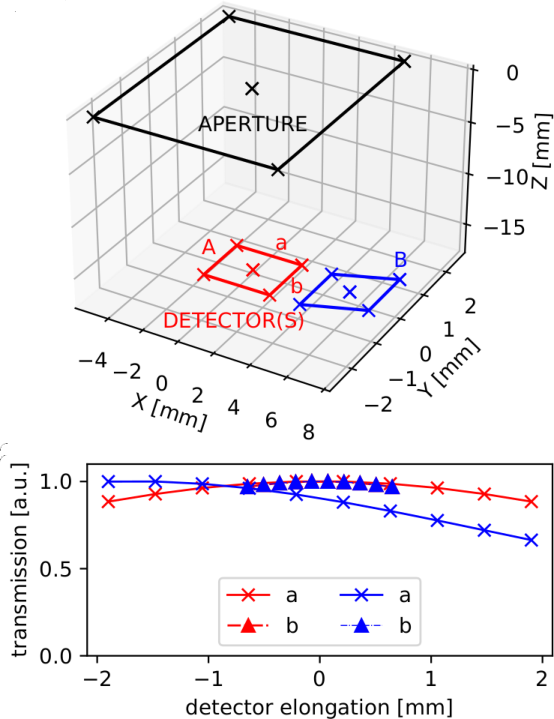
\includegraphics[width=\textwidth]{%
                        content/figures/chapter1/etendue_box_lines.pdf}%
                    \caption{Etendue}\label{fig:etendue_box}%
                \end{subfigure}%
                \hspace*{1.0cm}%
                \begin{subfigure}{0.5\textwidth}%
                    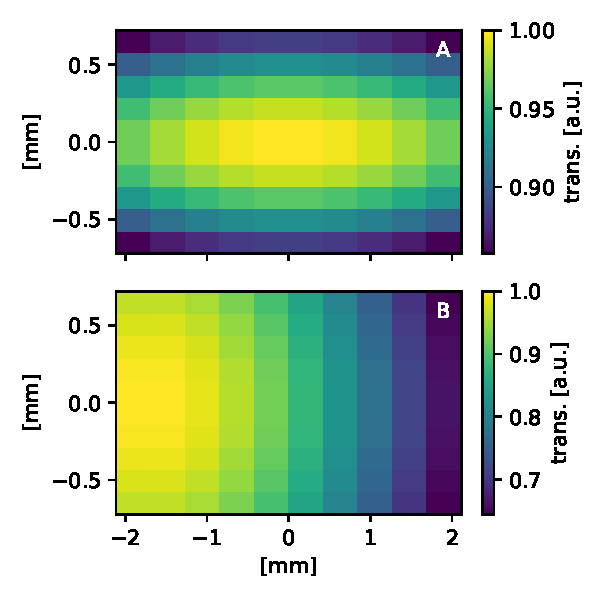
\includegraphics[width=\textwidth]{%
                        content/figures/chapter1/etendue_2D.pdf}%
                    \caption{Transmission}\label{fig:trans_map}%
                \end{subfigure}%
                \caption{\textbf{(a)}: (top) Detector $A$ and $B$ behind aperture with bolometer-like geometry. (bottom) Normalized transmission for both dimensions of the detectors. \textbf{(b)}: Map of the normalized etendue for both absorbers - top A and bottom B - on the left along $a$ and $b$. Their sizes and distances are representative of the W7-X bolometer.}\label{fig:etendue_transmission}%
            \end{figure}
%
            An example of how the transmission of a bolometer detector-pinhole pair looks like at W7-X can be seen in \cref{fig:etendue_transmission}. \autoref{eq:etendue_woline} has been numerically solved for an as-build combination, where both distances and orientations are the same as for the horizontal bolometer camera. Detector $A$ and $B$, as well as the aperture have been transformed into their own coordinate system for exemplary reasons. \autoref{fig:etendue_box} shows the general geometry with elongations of the detectors $a$ and $b$, as well as the transmission along those directions across the absorbers. The partial shadowing has a small impact on the light yield onto the outermost parts in the direction of the camera array, i.e. along $a$ towards $B$. However, perpendicular thereto the normalized transmission does not deviate. \autoref{fig:trans_map} combines these results in a map across the absorbers $A$ and $B$. The detector parallel to the aperture has a maximum in the center with varying gradients in both directions $a$ and $b$. Partial shadowing perpendicular to the lateral extent of the camera array has a stronger effect because of the orientation and dimensions of the aperture and detectors. The normalized yield onto absorber $B$ gradually decreases along $a$, i.e. further away from the pinhole. It is important to note that the exact details of this discussion change for the actual geometry of the VBC and HBC geometry.%
%
        \subsection{Bolometer Equations}\label{subsec:bolometerequations}%
%
            % Bolometer equations.
            In the following section the measurement principle of the metal resistive bolometer detector and the Wheatstone bridge will be introduced. Subsequently, the \textit{in-situ} calibration method, performed before every measurement, and its conclusions for the calculation of the radiation power onto the absorber will be outlined. Enclosed therein is a simplified derivation of the bolometer equation used to estimate the plasma radiation from the entire device, as well as a very general and exemplary approach to reproductions of local radiation distributions.%
%
            \subsubsection*{Measurement Principle}%
%
                \begin{figure}[t]%
                    \centering%
                    \begin{subfigure}{0.48\textwidth}%
                        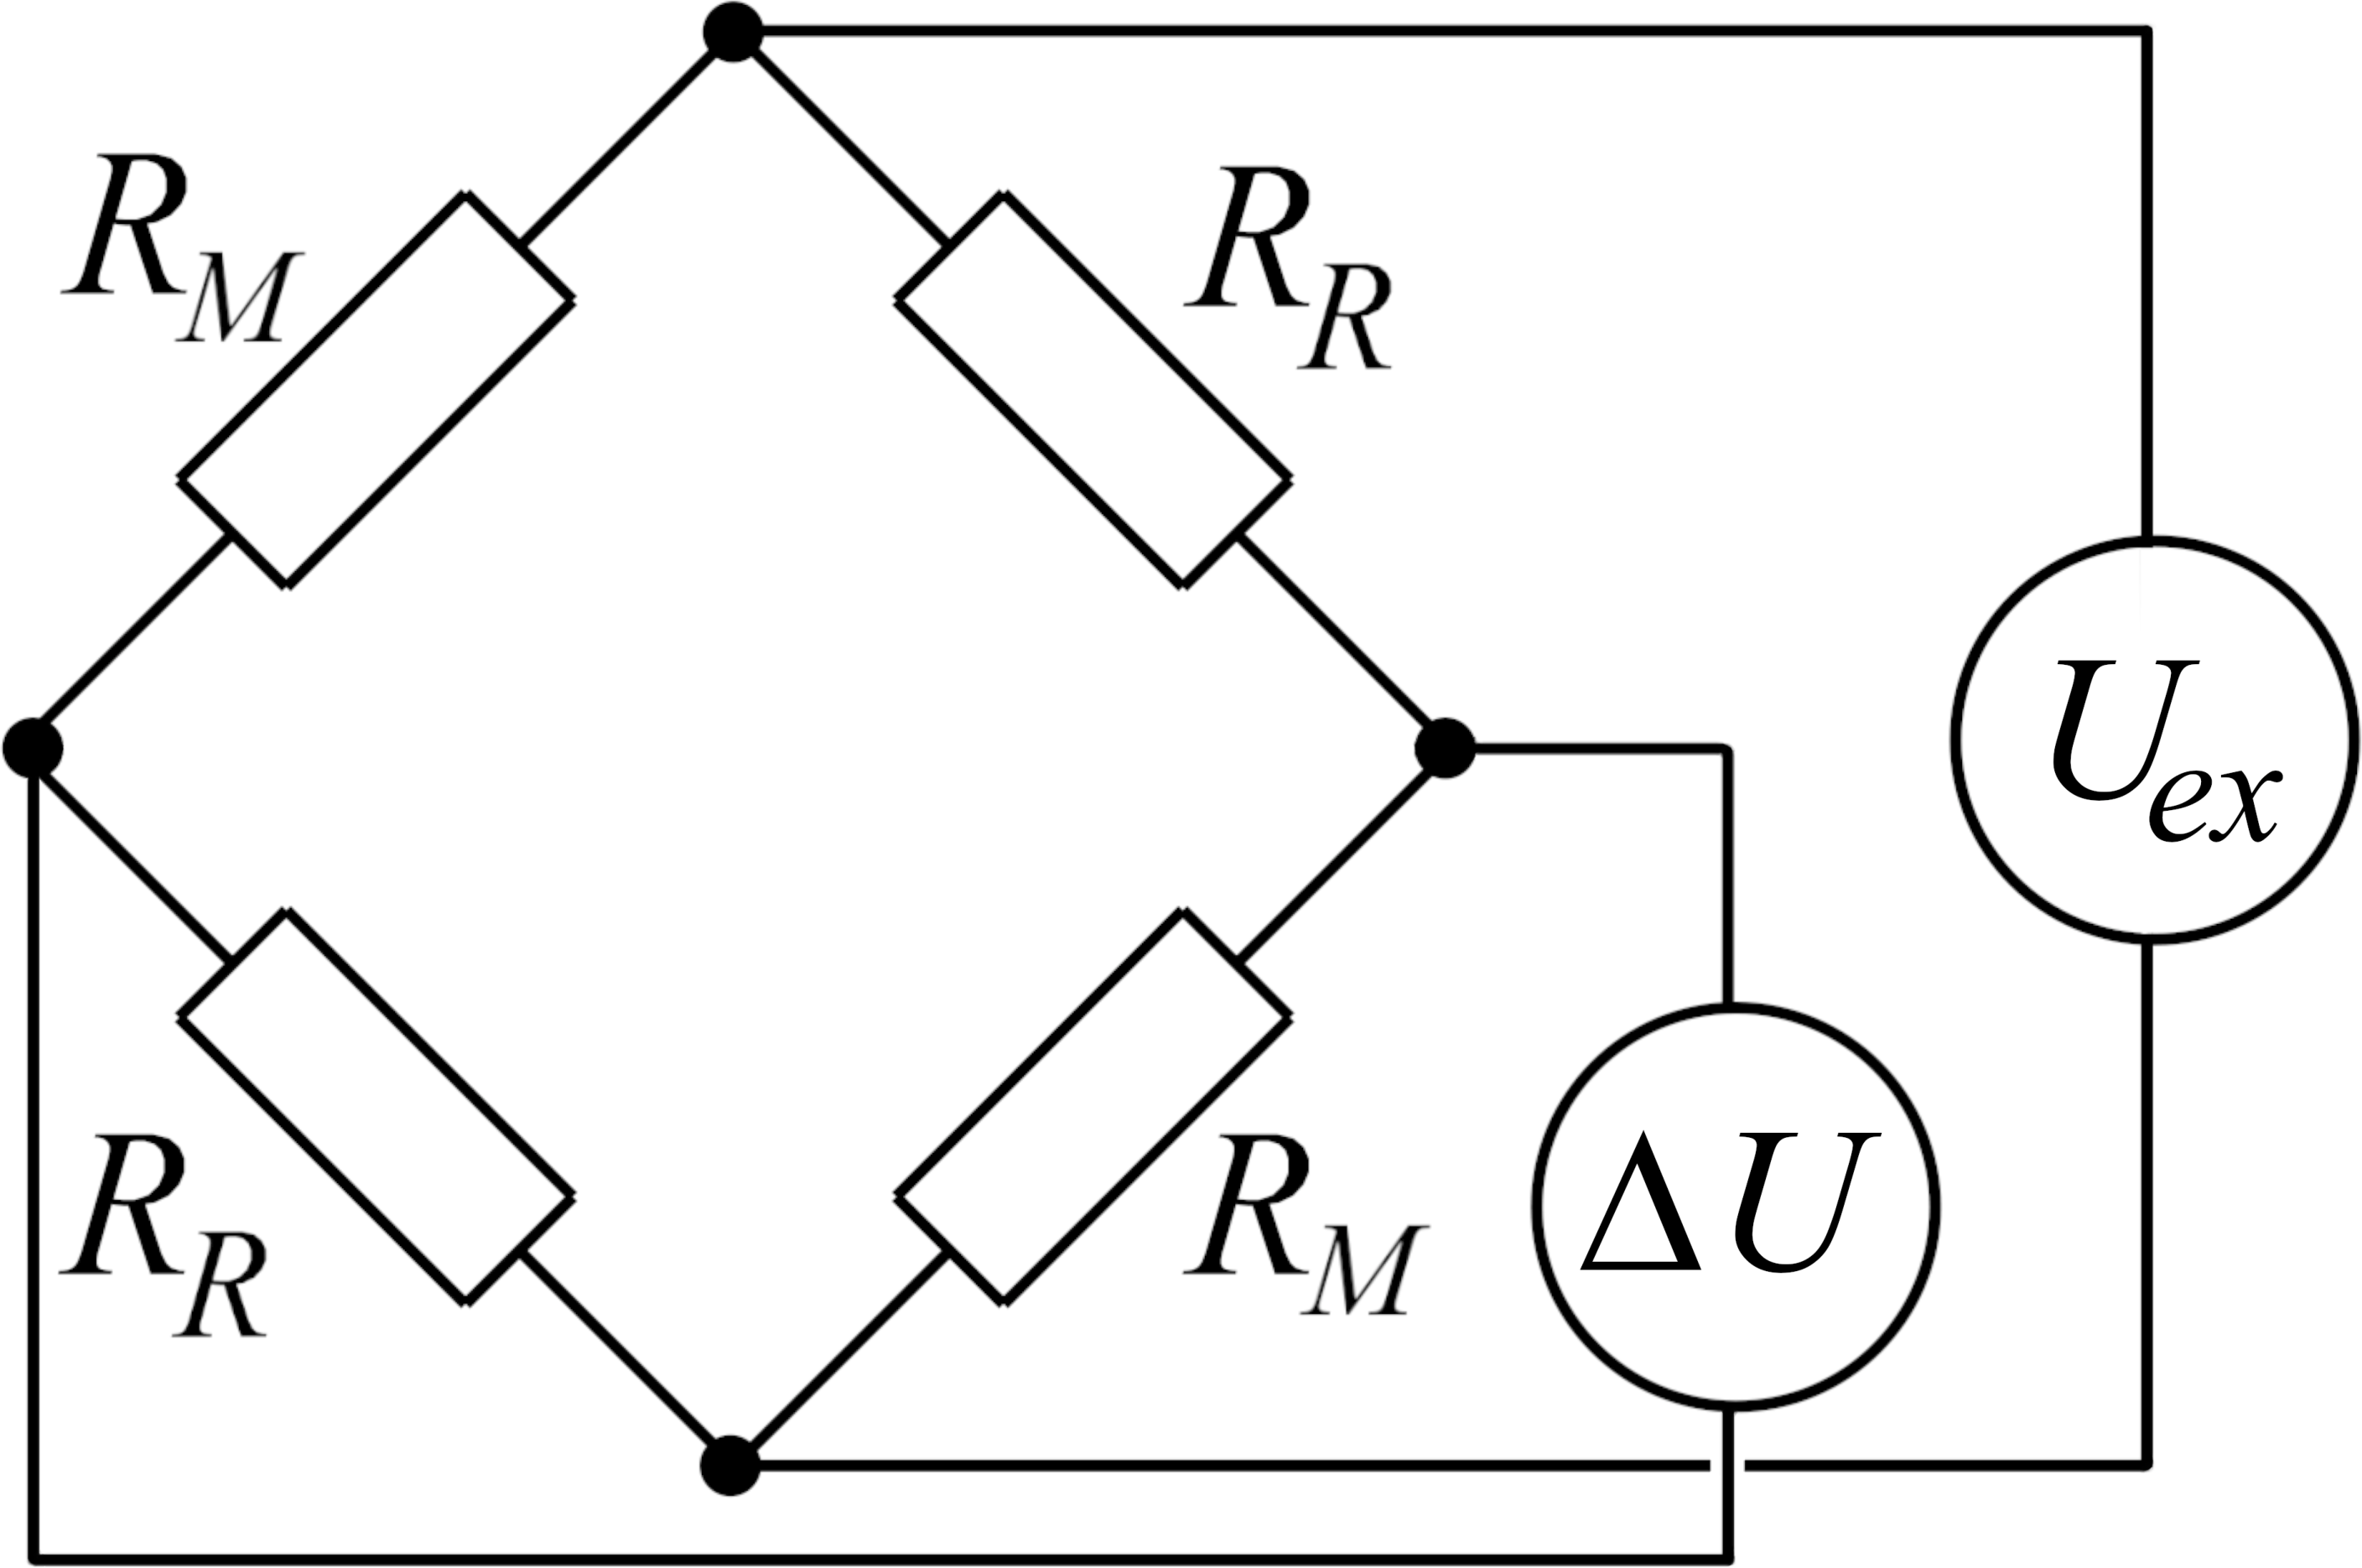
\includegraphics[width=\textwidth]{%
                            content/figures/chapter1/wheatstone3.pdf}%
                        \caption{Measurement}\label{fig:wheatstone}%
                    \end{subfigure}%
                    \hfill%
                    \begin{subfigure}{0.48\textwidth}%
                        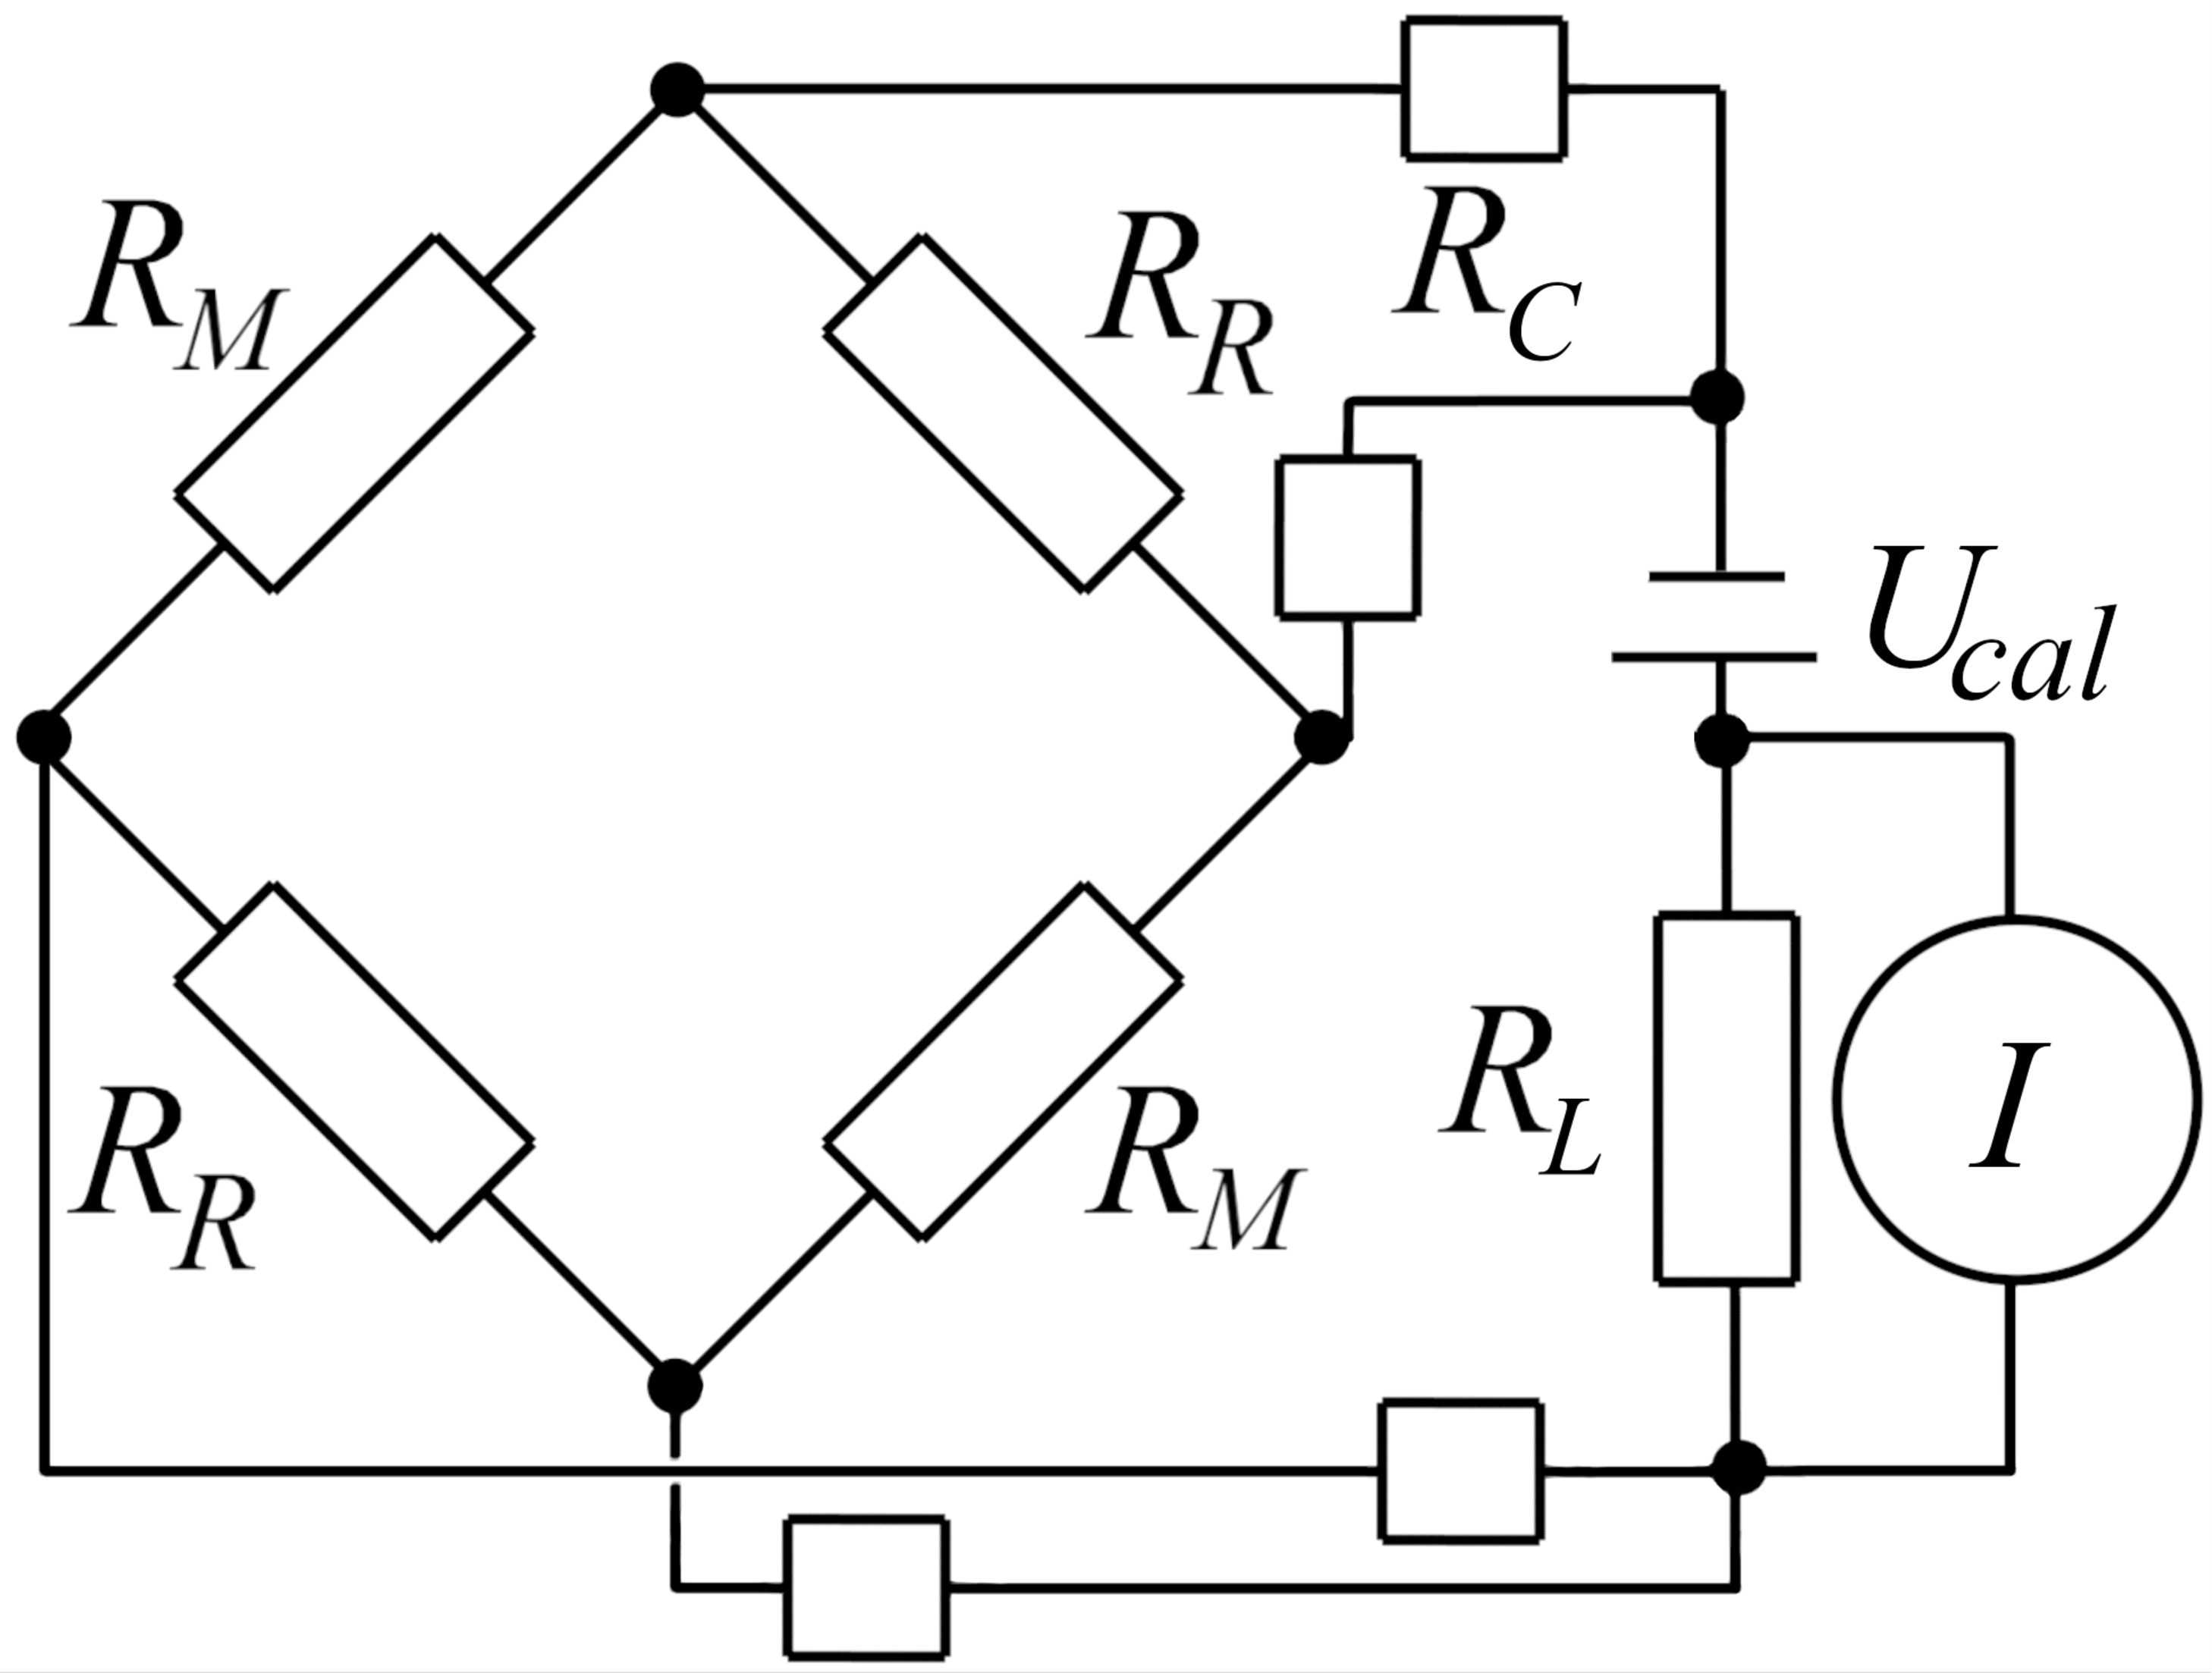
\includegraphics[width=\textwidth]{%
                            content/figures/chapter1/Wheatstone_calib3.pdf}%
                        \caption{Calibration}\label{fig:wheatstone_calib}%
                    \end{subfigure}%
                    \caption{\textbf{(a)}: Schematic Wheatstone bridge with measurement ($M$) and reference ($R$) resistors $R_{M}$ and $R_{R}$ respectively. Both are thermally linked to an absorber, while the measurement part only is exposed to incident power. The bridge is connected with a voltmeter and AC excitation source. \textbf{(b)}: Equivalent circuit for calibration of the Wheatstone bridge, with DC voltage $U\ix{cal}$, cable resistances $R\ix{C}$ and an additional load $R\ix{L}$ for current measurement $I$.}\label{fig:wheatstone_two}%
                \end{figure}%
%
                The electrical circuit schematic as an example can be seen in \cref{fig:wheatstone}. Measurement ($M$) absorbers are thermally connected to the $R_{M}$, whereas the non-exposed reference ($R$) detectors are connected to $R_{R}$. Generally the idea is to apply a large excitation voltage $U\ix{ex}$ across one \textit{diagonal} of the bridge and measuring the small resulting $\Delta U$ across the other. In a "dark" scenario one assumes $R_{M}=R_{R}=R$ both resistances to be equal and the bridge to be balanced, hence $\Delta U=0$. Through incident power the measurement absorber heats up, causing the temperature of $R_{M}$ to rise and its value to increase by $\Delta R$. For this unbalanced bridge one finds:%
%
                \begin{align}%
                    \frac{\Delta U}{U\ix{ex}}=\frac{R+\Delta R}{2R+\Delta R}-\frac{R}{2R+\Delta R}\approx\frac{\Delta R}{2R}\,\,.\label{eq:base_wheatstone}%
                \end{align}%
%
                Since the bridge balance is perturbed by the temperature change in both $R_{M}$ simultaneously, the signal-to-noise is doubled since the noise of the measurement is governed by external factors such as cables and acquisition electronics.\\%
                The excitation voltage $U\ix{ex}$ has an amplitude (AC) of \SI{5}{\volt}, with an adjustable frequency in the \SI{}{\kilo\hertz} range. Direct current (DC) coupled excitations are not well suited to this problem, since the already small resistance perturbation $\Delta R$ is superimposed by a dominating noise component that scales $\propto 1/f$ the frequency in the power spectrum\cite{Horowitz1989,Weissman1988}. When applying the AC current one measures the resistance at the frequency of the excitation and thereby removes a large uncertainty by discarding the rest of the spectrum.\\%
                At the bolometer diagnostic at W7-X, the bridge imbalance is directly measured as $\Delta U$ for an excitation cycle with the connected electric circuit including cables in mind. The equivalent circuit for such bridge measurements can be seen \cref{fig:wheatstone} and the conclusive \cref{eq:bolometer}. Derivations in respect thereof are largely based on the work provided by Giannone~et.~al\cite{Giannone2002}.\\%
%
                    \begin{figure}%[t]%
                        \centering%
                        \includegraphics[width=\textwidth]{%
                            content/figures/chapter1/signal_example_response.pdf}%
                        \caption{An example for a normalized single power stage of \SI{0.5}{\second} and resistive absorber response as described above. Shown on the left is the incident power. In the center are both the gain and time derivative of the voltage drop across the absorber. The final image on the right shows the sum of the latter, which again yields the input power.}\label{fig:signal_example}%
                    \end{figure}%
%
                After having defined the measurement voltage $\Delta U$ and resistance change $\Delta R$ for the detector one can now calculate the temperature change $\Delta T$ and consecutively incident power $P\ix{bolo}$ onto the absorber. For this assembly, particularly by design with Pt meanders, the detector resistance increases linearly with the temperature, i.e. $\hat{R}=\alpha R\Delta T$. The temperature change can be written using \cref{eq:base_wheatstone} in terms of $\Delta U$. Finally, the temperature change $\Delta T$ is given by the incident power $P\ix{bol}$, the heat capacity $\kappa$ and the cooling time $\tau$ of the absorber.%
%
                \begin{align}%
                    \begin{split}\label{eq:resistance_power}%
                        \Delta T&=\frac{\Delta R}{\hat{R}}=\frac{2\Delta U}{\alpha U\ix{ex}}\\%
                        \kappa\frac{\diff\left(\Delta T\right)}{\diff t}&=P\ix{bol}-\kappa\frac{\Delta T}{\tau}%
                    \end{split}\\%
                    P\ix{bol}&=\frac{2R\kappa}{U\ix{ex}\hat{R}\tau}\left(\Delta U+\tau\frac{\diff\left(\Delta U\right)}{\diff t}\right)\label{eq:bolopower}
                \end{align}%
%
                \autoref{eq:bolopower} only depends on the intrinsic characteristics of the absorber, i.e. its thermal properties and the measurement voltage $\Delta U$. The heat capacity $\kappa$ measures how much power the absorber can store. While the cooling time $\tau$ expresses the exponential rate and time constant at which the element dissipates heat. An example for this can be seen in \cref{fig:signal_example}: for a single stage of incident power, e.g. a heating pulse of microwaves, the sum of $\diff\left(\Delta U\right)/\diff t$ and $\diff\Delta U/\tau$ represents the input radiation (arbitrary units). While normalized quantities are shown in this figure, given that the thermal properties are known, i.e. heat capacity, cooling time etc., one can accurately calculate the power using this approach. In order to accurately calculate the bolometer detector power in practice one needs to calibrate the absorber and find its respective properties.% 
%
            \subsubsection*{Calibration}%
%
                A reliable, accurate, \textit{in-situ} calibration procedure is needed to find the total incident power onto the absorber. Because of manufacturing processes, no detector is created equal, especially with regard to layer and substrate thickness. Variations in absorber composition lead to changes in heat capacity, resistance or cooling time across a camera or even a single Wheatstone bridge. Also, deterioration due to exposition to heavy plasma radiation also might contribute to a change in response of the detector. Continuously monitoring the systems characteristics is key, especially in context of the application in this experiment. Therefore, a calibration method based off an \textit{Ohmic heating phase}, involving reference resistors for comparison and taking cable properties into account has been established and used in past experiment campaigns. One should note that this is, with minor changes, based off of the derivations made by Giannone~et al.\cite{Giannone2002}.\\%
                An equivalent circuit for the calibration of the previously discussed Wheatstone bridge can be seen in \cref{fig:wheatstone_calib}. Two concurrent voltage levels are applied to either the two measurement or reference resistors, while the respective others are short-circuited. The NI\textsuperscript{\textregistered} AD7300 is capable of both voltage and current measurement - although consecutively and not in parallel. An example of two current stages for one pair of measurement and reference resistor from the same Wheatstone bridge can be seen in \cref{fig:ohmicheating}.\\%
%
                \begin{figure}[t]%
                    \centering%
                    \includegraphics[width=0.7\textwidth]{%
                        content/figures/chapter1/%
                        heating_ohmic_example_full.pdf}\\%
                    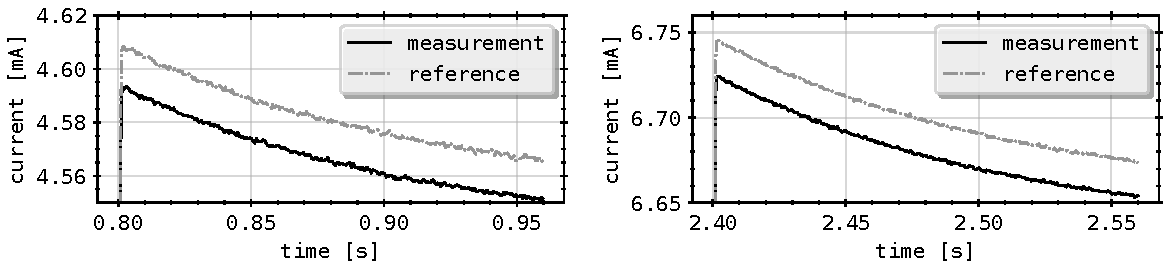
\includegraphics[width=.9\textwidth]{%
                        content/figures/chapter1/heating_ohmic_example_ch0.pdf}%
                    \caption{Example of the first (left) and second (right, both - top) Ohmic heating stages as described for measurement and reference absorbers. One easily notices the difference in absorber response between reference and measurement part of the same bridge. The maximum current before the exponential decay during the first heating pulse corresponds to $\Delta I\left(0\right)$.}\label{fig:ohmicheating}%
                \end{figure}%
%
                First, the current flowing through the resistor at floating potential $I_{0}$ is measured as a baseline. It is assumed that element $M$ has the resistance $R_{M}$ before the calibration. For two values of $U\ix{cal}=\SI{1.2}{\volt}$ and \SI{2.5}{\volt} the stages are run each for \SI{1.6}{\second}. The current through the resistor evolves with $I\left(t\right)$ and eventually equilibrates, i.e. $t\rightarrow\infty$.
                One therefore finds for the resistance from the current in the first stage:%
%
                \begin{align}%
                    R_{M}=2\left(\frac{U\ix{cal}}{I\left(t\rightarrow\infty\right)-I_{0}}-R\ix{L}-R\ix{C}\right)\,\,.\label{eq:resistance}%
                \end{align}%
%
                Here, $R\ix{L}=\SI{10}{\ohm}$ is an additional load resistor in the acquisition circuit outside the Wheatstone bridge and $R\ix{C}=\SI{40}{\ohm}$ accounts for the connected cables. The electric power leads to an Ohmic heating of the foil, increasing the temperature, which, due to a temperature change of the resistor, changes the resistance and therefore again the current flowing through the detector. One assumes a current perturbation due to the Ohmic heating $\Delta I\left(t\right)$ to be superimposed onto $I\left(t\right)$. The cooling time rate towards equilibrium, i.e. $\Delta I\rightarrow 0$ can be expressed by an exponential decay function:%
%
                \begin{align}%
                    \Delta I\left(t\right)=-\Delta I\left(0\right)\left[1-\exp\left(-\frac{t}{\tau_{M}}\right)\right]\,\,.\label{eq:timedecay}%
                \end{align}%
%
                Here, $\tau_{M}$ yields the temperature decay or cooling time constant of the resistor $M$. The time $t$ is measured relative to the occurrence of the ohmic heating stage, and $\Delta I\left(0\right)$ is the resulting maximum current thereof. By a numeric fitting procedure of the previous function in \cref{eq:timedecay} to the response of the detector one easily finds the values of $\tau_{M}$ and $\Delta I\left(0\right)$.\\%
                Differences in foil and substrate thicknesses result in different heat capacities $\kappa$ of each absorber, while the thermal contacting to the body of the bolometer chip holder also varies and results in variations in cooling time $\tau$. Hence, the initial response to the Ohmic heating stage can be significantly different to an exponential decay. However, the cooling is dominated by the carbon coated gold and aluminium layer in-between. Therefore, the first few milliseconds of the heating stage are excluded from the numerical fit of the function in \cref{eq:timedecay} in order to find $\tau$ and $\kappa$. Important to note is that in this case, the change of the current $I\left(t\right)$ does not yield the maximum current through the detector, as noted above by $\Delta I\left(0\right)$. This property is measured independently at the peak of $I\left(t\right)$ during the Ohmic heating pulse.\\%
                The current when heated up $\Delta I\left(0\right)$ can be used the find the (normalized) heat capacity $\kappa_{M}$. By linearization of the change $\Delta R$ in resistor value $R_{M}$ one can write the power balance during the current stage as:%
%
                \begin{align}%
                    \begin{split}\label{eq:powerbalance}%
                        \frac{U\ix{cal}I^{2}_{0}}{I\left(\infty\right)-I_{0}}+\frac{I\left(\infty\right)I_{0}R_{M}}{2}=-\kappa_{M}\frac{4U\ix{cal}}{I^{2}_{0}}\left[\frac{\diff\Delta I}{\diff t}+\Delta I\right]\,\,.%
                    \end{split}%
                \end{align}%
%
                Substituting \cref{eq:timedecay} for $\Delta I$ and calculating for the steady state case, i.e. $t\rightarrow\infty$ hence $\diff I/\diff t\rightarrow 0$ and $\Delta I\rightarrow 0$, \cref{eq:powerbalance} can be rewritten to:%
%
                \begin{align}%
                    \kappa_{M}=\frac{\Delta I^{4}\left(0\right)}{4I\left(\infty\right)\left(I\left(\infty\right)-I_{0}\right)}\,\,.\label{eq:heatcapacity}%
                \end{align}%
%
                \begin{figure}[t]%
                    \centering%
                    \includegraphics[width=\textwidth]{%
                        content/figures/chapter1/calibs_example.pdf}
                    \caption{Example for a set of calculated normalized heat capacities, resistances and cooling times for both measurement and reference detectors as described below. Small groups of four consecutive detectors in each property hints at similarities in composition irregularity. Reference channel number 32 in the middle figure shows an especially low heat capacity, indicating an issue with the thermal contact of the meander bridge.}\label{fig:calibsexample}%
                \end{figure}%
%
                With the previously outlined setup it is possible to do the above measurements for all measurement and reference resistors of the Wheatstone bridge, which results in the values of $\tau$, $\kappa$ and $R$ for each individually. Those are important not only for the calculation of the plasma radiation power, but for information on detector status and reliability as well. An example for a set of calculated $\kappa$, $R$ and $\tau$ for both exposed and hidden counterparts can be seen in \cref{fig:calibsexample}.\\%
                \,\\%
%
                In reality, the above equations have to be corrected to account for the temperature dependence of all three quantities.  This has not been pursued for the bolometer system at hand. Furthermore, Zhang~et al. addressed the influence\cite{Zhang2009} of ambient pressures and concluded, that an increase of up to \SI{20}{\pascal} leads to an equivalent, non-negligible pseudo signal of \SIrange{2}{8}{\watt\per\meter\square\per\pascal}, while the expected change in pressure during experiments is \SIrange{0.5}{10}{\pascal}. However, the expected maximum pressure of plasma discharges in W7-X is $\approx\SI{1e-2}{\pascal}$, therefore this is not an issue. Tests in \textit{VINETA}\footnote[1]{VINETA: Versatile Instrument for Studies on Nonlinearity, Electromagnetism, Turbulence and Application} have found that the detector characteristic is susceptible to strong ambient pressure and temperature changes. A \textit{strain-gauge} factor as a function of the resistivity and pressure was defined, which was found to have a hysteresis and change with the line integrated power\cite{Zhang2008}. Nevertheless, one would need an individual gauge to measure local baseline pressures or flow rates through or at the pinhole to most accurately address this problem. Another approach would be to install one or more blind absorbers that are not exposed, so they can be used to subtract a bias from the signals of the corresponding camera.\\%
                For the validity of the bolometer measurements its performance under conditions of high neutral gas density is of concern, where an additional component of the bolometer signal comes from localized, high energy neutral particles from charge exchange processes at the plasma edge. First order corrections to the bolometer equations can be made by incorporating neutral gas simulation codes with charge exchange to numerical simulations of the measurement\cite{Giannone1997}. This has not been exercised for the bolometer at W7-X.\\%
                The expected \SI{10}{\kilo\watt\per\square\meter} high thermal loads on plasma facing components and conclusive temperature perturbations of the camera enclosure of the bolometer may lead to additional signal drifts due to infrared radiation from inside the diagnostic housing. As a simplest estimate of \textit{grey body radiation}, such a drift is $\propto \varepsilon A\Delta T^{4}$ according to the \textit{Stefan-Boltzmann\footnote[1]{Jožef Štefan *~Mar. 24, 1835 \textdagger~Jan. 7, 1893}$^{, }$\footnote[2]{Ludwig Eduard Boltzman *~Feb. 20, 1844 \textdagger~ Sep. 5, 1906} law}, where $A$ is the surface area of the insides of the camera housing, $\Delta T$ the relative temperature change to a baseline and $\varepsilon$ an emissivity efficiency. In a more accurate model this is in fact frequency dependent with $\varepsilon\left(\nu\right)$, since the camera enclosure is not adequate described as a black body. To add to that, perturbations of the integrated camera holder water cooling have also presented strong, thermally induced signal drifts. An example for this can be seen in \cref{fig:tempdrift}.\\%
                Previously, Zhang~et al. have modelled the temperature impact on detector properties for the above equations\cite{Zhang2012}. It was concluded that the detector characteristics become functions of the temperature increments in all parts of the bridge, i.e. $\Delta T_{M}$ and $\Delta T_{R}$ of measurement and reference absorber respectively, and that the major impact on signal form is imposed by thermal changes in the resistance $R$ and heat capacity $\kappa$. It was found that the drift and offset are in the range of \SIrange{50}{150}{\micro\volt\per\kelvin}, depending on the composition of the absorber\cite{Zhang2012}. A simultaneous measurement of both bridge voltage $\Delta U$ and current through the Wheatstone bridge for parallel data acquisition and calibration has not been implemented. The similarly designed bolometer at the future large tokamak fusion device ITER will feature a real-time calibration parallel to data acquisition\cite{Penzel2017}.\\%
%
                \begin{figure}[t]%
                    \centering%
                    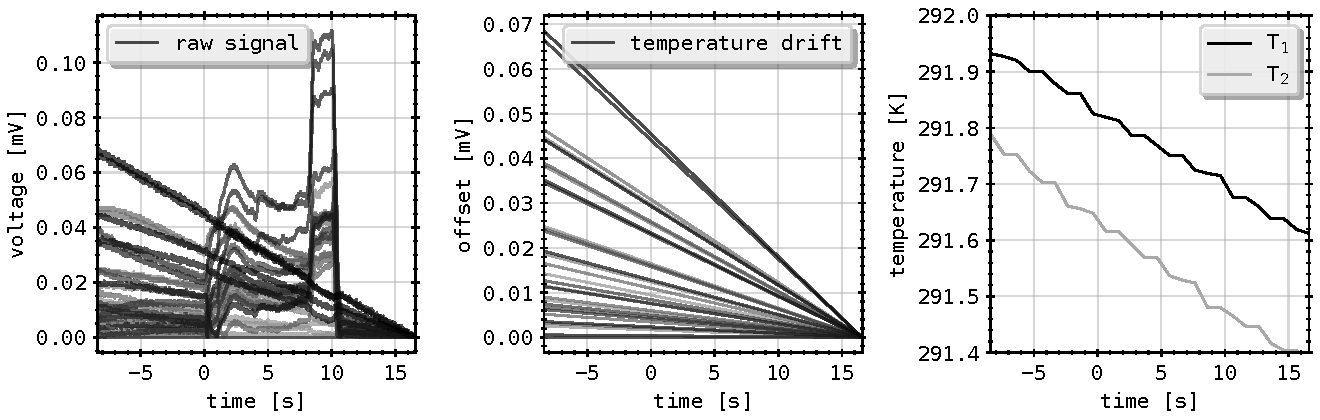
\includegraphics[width=\textwidth]{%
                        content/figures/chapter1/temperature_drift.pdf}%
                    \caption{The left image shows the unaltered detector signal as measured by the data acquisition for the main HBC array in the W7-X experiment XP20180927.37. The middle is the subtracted, assuming linear, temperature drift for each of those channels. Note how either every channel has different drift functions or entirely different temperatures. The right picture shows the measurement results of two \textit{Pt100} resistive thermometers from the back of the HBC array over the course of the experiment}\label{fig:tempdrift}%
                \end{figure}%
%
                For long pulse experiments this issue can be avoided by systematically looking up known calibration values at given absorber temperatures and ambient pressures. The future \textit{divertor bolometer system} at W7-X will pursue this strategy. As further reference, the literature notes the change in heat capacity, cooling time and resistance of a gold with a rate of \SI{25}{\joule\per\kelvin\per\mol}, \SI{0.13}{\milli\second\per\kelvin} and \SI{0.008}{\nano\ohm\meter\per\kelvin} respectively. This behaviour is mostly linear beyond a threshold of \SI{275}{\kelvin}\cite{Takahashi1986,Cutnell1998,Lloyd1998,Seitz1987,Lide1996}. This again underlines the necessity of active cooling of the bolometer camera. \\%
                The temperature increase of the resistor and absorber due to voltages applied for excitation during the measurement process is expected to be \SI{25}{\kelvin}. The calibration itself also heats up the foil through the Ohmic heating phase. It can be assumed that the increase in temperature is similar during both and this effect will be neglected in later considerations\cite{Zhang2012}. The future divertor bolometer will conduct absorber calibrations while also applying the measurement excitation.%
%
            \subsubsection*{Radiation Power Measurement}%
%
                After a successfully performed calibration the power onto the absorber can be calculated. Following will be an outline of this process, accompanying the equations to calculate the incident radiation power.\\%
                In general, the radiation from the plasma along the line of sight (LOS) of an absorber can be written as:%
%
                \begin{align}%
                    P\ix{rad}\propto\int_{LOS}\sum_{Z}n_{e}\cdot n_{Z}\cdot L_{Z}\left(T_{e}, T_{i}, T_{Z},\,\,\dots\right)\frac{\diff l}{4\pi}\,\,.\label{eq:lineradiation}%
                \end{align}%
%
                Here, $P_{rad}$ shall be the total incident power as measured by the bolometer absorber. This is, in theory, proportional to the sum over all \textit{(line) radiation functions} $L_{Z}$ of elements $Z$, which describes the combined emission from both continuum and atomic processes at a given set of plasma parameters, e.g. electron and ion temperature $T_{e,i}$, as well as the condition of the device.\\%
                Consider that $\Delta U$ the output voltage of the Wheatstone bridge is being measured in the equivalent circuit shown in \cref{fig:wheatstone}. In accordance to \cref{eq:bolopower} the radiation power onto the measurement absorber can be expressed in $P\ix{bol}$. Adjusting \cref{eq:bolopower} to the details of the measurement circuit for absorber $M$ of the Wendelstein 7-X bolometer diagnostic, one arrives at the \tilt{bolometer equation}:%
%
                \begin{align}%
                        \widetilde{P}_{M}=\frac{2}{V\ix{eff}}&\left(R_{M}+2R\ix{C}\right)\kappa_{M}\sqrt{g\ix{C}}\left(\tau_{M}\frac{\diff(\Delta U_{M})}{\diff t}+f_{\tau}\Delta U_{M}\right)\,\,.\label{eq:bolometer}%
                \end{align}%
%
                The corresponding parameters of the data acquisition setup for \cref{eq:bolometer}, i.e. $V\ix{eff}$, $f_{\tau}$, $g\ix{C}$, $\beta$, $\omega$ etc. are shown below in \cref{eq:bolometer_variables}. The variable Wheatstone bridge frequency $f\ix{bridge}$ is commonly set to $\frac{1}{\text{\SI{0.8}{\milli\second}}}=$\SI{1250}{\hertz} or $\frac{1}{\text{\SI{1.6}{\milli\second}}}=\,$\SI{625}{\hertz} and cable parameters are measured to be $R\ix{C}=\text{\SI{40}{\ohm}}$ and $C\ix{C}=\text{\SI{2}{\nano\farad}}$ respectively.%
%
                \begin{align}
                    \begin{split}\label{eq:bolometer_variables}
                        V\ix{eff}&=\frac{\left(\text{\SI{5}{\volt}}\right)\cdot\,R_{M}}{R_{M}+2R\ix{C}}\\%
                        g\ix{C}&=1+\left(\omega\left(R_{M}+R\ix{C}\right)\right)^{2}\\%
                        \beta&=\frac{1-\left(\omega R_{M}\right)^{2}+\left(\omega R\ix{C}\right)^{2}}{1+\left(\omega\cdot\left(R_{M}+R\ix{C}\right)\right)^{2}}\\%
                        \omega&=2\pi\cdot f\ix{bridge}C\ix{C}\\%
                        f_\tau&=1-\frac{V\ix{eff}^{2}\cdot\beta}{4\kappa\ix{M}\left(R_{M}+R\ix{C}\right)^{2}}%
                    \end{split}
                \end{align}
%
                As previously pointed out, \cref{eq:bolometer} is only a valid estimator for the radiation power in a single detector within a small temperature range and at constant neutral gas pressures. During manometer tests where the vessel pressure was continuously increased, detector signals rose in the absence of plasma or radiation. Additionally, each detector is only accepted for evaluation if its calibration values are within a 3\% deviation window from their reference counterpart.\\%
                In summary, the absorbed radiated power is expressed as a function of voltage drop across the Wheatstone bridge as shown in absorber and the corresponding time derivative. Assuming $R_{M}\approx\text{\SI{1}{\kilo\ohm}}$, $\tau_{M}\approx\text{\SI{110}{\milli\second}}$ and $\kappa_{M}\approx\text{\SI{0.8}{\milli\watt/\kilo\ohm}}$, which gives $\omega=\text{\SI{3.14e-5}{\hertz\farad}}$, $\beta\approx1$, $\sqrt{g\ix{C}}\approx1$, $V\ix{eff}=\text{\SI{4.63}{\volt}}$ and $f_{\tau}\approx1$, \cref{eq:bolopower} can be written for a sample time of \SI{1.6}{\milli\second} as:%
%
                \begin{align}%
                    \widetilde{P}_{M}\approx\text{\SI{25.74}{\watt\per\volt}}\left(\diff(\Delta U_{M})+0.014\Delta U_{M}\right)\,\,.\label{eq:approx}%
                \end{align}%
%
                Commonly one finds during a measurement of plasma radiation at W7-X $\Delta U\sim\text{\SI{e-3}{\volt}}$ and the change in signal on the time basis given above $\diff(\Delta U)\sim\text{\SI{e-5}{\volt}}$. Hence, the predominant part of the equation is the raw signal, however during transient phases with fast changes of plasma radiation distribution the dynamic part may play a more important role therefore set the time resolution of the system by requirements regarding the signal-to-noise ratio.\\%
                The raw signal has to be offset corrected. e.g. for temperature drifts. By design of the system, the detector temperature changes naturally due to ohmic heating by the excitation voltage and incident radiation. The calibration process however already saturates the absorber temperature through ohmic heating, so that an additional heating during the actual measurement is not experienced. External thermal interference through the perturbations of the water cooling and heating of the camera enclosure (and other plasma facing components) and subsequent infrared radiation also may add to possible thermal drifts or signal errors.\\%
                In summary, the baseline offset is calculated from the mean voltage $\Delta U$ in the first few (hundred) milliseconds of measurement before plasma startup at $T_{0}$ in order to account for an initial imbalance of the Wheatstone bridge before the experiment.%
%
                \begin{align}%
                    V\ix{off}=\frac{1}{t_{2}-t_{1}}\int_{t_{1}}^{t_{2}}\Delta U_{M}\left(t\right)\diff t\,\,\,,\,\,t_{1}<t_{2}<T_{0}\label{eq:offset}
                \end{align}%
%
                An expected temperature and signal drift is compensated using the \textit{least squares} method to fit a linear function $f\left(t, \beta_{1}, \beta_{2}\right)$ as offset between the detector signal before the start and end of experiment. This approach is based on the assumption of linearity in first order temperature dependency of the calibration properties, as well as a slow linear temperature rise due to a large enough thermal inertia or reservoir of the machine. Data points beyond the end of the experiment, where incident radiation no longer heats up the absorber, are not included since the detector already begins to exponentially cool down. Let $t_{1}$ be the point in time just before the start of the plasma heating, $t_{2}$ right after it shutting off and $\overline{\Delta U}\left(t\right)$ be a 50\,-100 sample median of the signal around $t$. Then $\vec{\beta}=\left(\beta_{1}, \beta_{2}\right)$, $\vec{f}=\left(f\left(t_{1},\vec{\beta}\right), f\left(t_{2}, \vec{\beta}\right)\right)$, $\vec{\Delta U_{M}}=\left(\overline{\Delta U}_{M}\left(t_{1}\right), \overline{\Delta U}_{M}\left(t_{2}\right)\right)$ become the component forms of the parameters, fit and target function at those given times. The drift problem therefore is:%
%
                \begin{align}%
                    \begin{split}\label{eq:linear_fit}%
                        r_{i}=&\Delta U\ix{M}\left(t_{i}\right)-f\left(t_{i},\beta_{1}, \beta_{2}\right)\\%
                        R\ix{res}=&\sum_{i=1}^{n}r_{i}^{2}=\|\vec{f}\left(t, \vec{\beta}\right)-\vec{\Delta U\ix{M}}\|\\%
                        &\underset{\vec{\beta}}{\text{argmin}}\left[\|\vec{f}\left(t, \vec{\beta}\right)-\vec{\Delta U\ix{M}}\|\right]%
                    \end{split}%
                \end{align}%
% 
                Solving the minimization problem in \cref{eq:linear_fit}, given that $\beta_{i}\in\mathbb{R}^{+}$ are positive for direct proportionality between the absorber response and temperature, one yields:%
%
                \begin{align}%
                    V\ix{drift}\left(t\right)=&\left\{%
                    \begin{array}{ll}%
                        0&,\,\,t<t_{1}\,\&\,t>t_{2}\\%
                        \beta_{1}\cdot t+\beta_{2}&,\,\,\text{else}%
                    \end{array}\right.\label{eq:drift}%
                \end{align}%
%
                Let the resulting signal, i.e. offset- and drift-corrected be $\Delta U^{*}_{M}$. To save one step in calculation, one can easily see that $\beta_{2}=0$ either becomes zero for an offset-corrected $\Delta U_{M}$ as a training set, or $\beta_{2}=V\ix{off}$ else. Additionally, the latter approach ensures that $\Delta U^{*}_{M}\approx0$ around $T=T_{0}$ where no plasma radiation or thermal interference is expected.\\%
                To avoid larger contributions of the derivative term $\diff\left(\Delta U^{*}_{M}\right)/\diff t$ for small $\diff t$ or large signal noise one applies a filter. A frequency gate via a low pass \textit{Savitzky Golay} polynomial fit of order $p$ and width $N$ or boxcar filter (moving mean) of width $N$ have been successfully tested and deployed with similar, adequate results. The filtered, \textit{corrected} voltage becomes $\Delta\widetilde{U}_{M}$. In the discretized, i.e. analog-to-digital converted  case, the $j$-th sample at time $t_{j}$ of $\Delta\widetilde{U}_{M}$ becomes a convolution of $N$ surrounding points with coefficients $c_{i}$ weighting the corrected data. In the case of the Savitzky Golay filter the coefficients $c_{i}=g\left(\Delta U_{M}^{*}\right)$ become a function of the convoluted signal, %
%
                \begin{align}%
                    \begin{split}%
                        \Delta\widetilde{U}_{M,j}=&\sum_{i=\frac{1-N}{2}}^{\frac{N-1}{2}}c_{i}\Delta U^{*}_{M, j+i}\\%
                        c_{i}=&\left\{\begin{array}{ll}%
                            1/N&,\,\text{boxcar}\\%
                            \frac{-3}{35},\,\frac{12}{35},\,\frac{17}{35},\,\frac{12}{35},\,\frac{-3}{35}&,\,i=\left\{-2,\dots2\right\}\text{S. G.}%
                        \end{array}\right.%
                    \end{split}\label{eq:averaging}%
                \end{align}%
%
                Finally, starting from \cref{eq:bolometer} and combining prefixes into detector specific factors, i.e. $F_{M}$ and $f_{M}$, as well as applying \cref{eq:drift} and \cref{eq:averaging}, one yields:%
%
                \begin{align}%
                    \begin{split}%
                        F_{M}=&\frac{2\tau_{M}}{V\ix{eff}}\left(R_{M}+2R\ix{C}\right)\kappa_{M}\sqrt{g\ix{C}}\,\,,\quad f_{M}=\frac{f_{\tau}}{\tau_{M}}\\%
                        \Aboxed{%
                            P_{M}\coloneqq&\widetilde{P}_{M}\left(\Delta\widetilde{U}_{M}\right)=F_{M}\cdot\left(\frac{\diff\left(\Delta\widetilde{U}_{M}\right)}{\diff t}+f_{M}\Delta\widetilde{U}_{M}\right)
                        }%
                    \end{split}\label{eq:bolometer_adv}%
                \end{align}%
%
                The \cref{eq:bolometer_adv} is the final form of the bolometer \cref{eq:bolopower} as it has been used in the past at the stellarator Wendelstein 7-X and will be during the course of this thesis for the results shown further below. \autoref{eq:bolometer_adv} is also again only a function of the absorber specific properties $F_{M}$ and $f_{M}$, as well as the post-processed Wheatstone bridge imbalance measurement $\Delta U$.%
%
        \subsection{Performance}\label{subsec:performance}%
%
            % Performance outline.
            The efficiency of gold absorbers has previously been found to be close in an absolute wavelength range between \SIrange{1e3}{1}{\nano\meter} to black nickel layer coatings\cite{Lang1996}. Meister~et.~al\cite{Meister2013} have measured the photoresponse of pure thin film platin absorbers of varying thickness, which are very similar to the carbon blackend gold film detectors at W7-X, and compared their results to photoabsorption calculations by Henke~et.~al\cite{Henke1993} for atomic (crystal) scattering, reflection and transmission. The results are shown in \cref{fig:pt_absorber}. From those tabulated results, this bolometer absorbers relative absorption efficiency is calculated and shown in \cref{fig:absorp_effic}. The efficiency with the highest uncertainties correlate to measurements at the lowest powers of the radiation source - channel no.1 and channel no.4 with respective thickness of \SI{9.7}{\micro\meter} and \SI{4.4}{\micro\meter}. The continuous, dashed and dotted-dashed black line are achieved by atomic scattering calculations\cite{Henke1993,Palik1997}. The obtained results of a thick absorber for photon energies above \SI{200}{\electronvolt} agree within their uncertainties with the literature. Efficiencies obtained for a thin absorber also matches but shows slightly lower values. The photoresponse of a \SI{5}{\micro\meter} thick gold absorber is therefore assumed to be unity in the range of \SIrange{600}{0.2}{\nano\meter}, where reflectivity is greatly reduced due to the coating, while the sensitivity of \SI{200}{\nano\watt} is still low. This provides the capability of absolutely calibrated measurements of the expected plasma radiation at W7-X.\\%
            The silicon frame and aluminium layer are used as thermal contact to diffuse the power load from the sensitive gold film resistor onto the graphite and stainless steel camera housing in order to limit the detector from reaching its maximum allowable temperature of \SI{250}{\celsius}.\\%
%
            \begin{figure}[t]%
                \centering%
                \begin{subfigure}{0.53\textwidth}%
                    \raisebox{1cm}{%
                        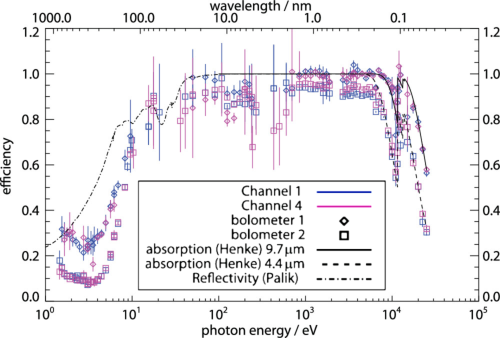
\includegraphics[width=\textwidth]{%
                            content/figures/chapter1/meister_sense.pdf}}%
                    \caption{Pt absorber\cite{Meister2013}}\label{fig:pt_absorber}%
                \end{subfigure}%
                \hspace*{0.75cm}%
                \begin{subfigure}{0.375\textwidth}%
                    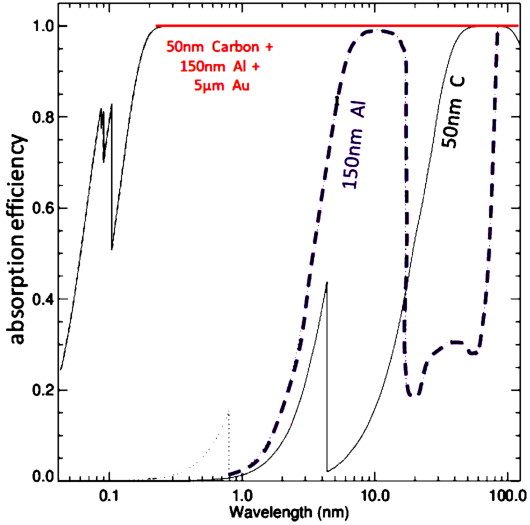
\includegraphics[width=\textwidth]{%
                        content/figures/chapter1/absorption_efficiency_full_detector.pdf}%
                    \caption{W7-X detector\cite{Zhang2024}}\label{fig:absorp_effic}%
                \end{subfigure}%
                \caption{\textbf{(a)}: Efficiency of bolometer absorber over incident photon energy as derived and measured by Meister~et.~al\cite{Meister2013}. \textbf{(b)} Relative absorption efficiency for full absorber assembly as shown in \cref{fig:detector_me}}\label{fig:sensitivity_meister}%
            \end{figure}%
%
            As previously mentioned, the bolometer diagnostic is required to manage at least \SI{10}{\kilo\watt\per\square\meter} of microwave stray radiation at its plasma facing front plate without degradation of the actual measurement. Therefore, any of the four detector arrays - two per camera each - are covered by a conductive wire-mesh of \SI{90}{\micro\meter} thickness and \SI{0.24}{\milli\meter} rectangular spacing in order to reduce the impact of non-absorbed microwave radiation through the pinhole. The optical transmission changes with detector location for the HBC because of differences in angle between line of sight and wire mesh normal, which reduces the light yield onto each absorber. However, this is not the case for both vertical camera arrays, where the arrangement is mounted individually directly in front of the subarrays. The resulting total optical transmission can be seen in \cref{fig:ftran}. The insides of the cameras have been coated with a special ceramic titanium oxide and aluminium oxide layer to enhance the microwave absorbance of the camera body and reduce the reflectance thereof. Additionally, special copper beryllium springs in the camera front plate mounting ensure a tight fit of the plasma facing component to reduce leakage of microwave radiation. Coating, holding plate springs and wire mesh all greatly improve the cameras' response to the microwave ECRH stray radiation\cite{Hirsch2013,Floristan2011}. Long duration tests with \SI{140}{\giga\hertz} strayfield microwave radiation onto the camera body and detector housing have been performed in MISTRAL\footnote[1]{MISTRAL: MIcrowave STray RAdiation Launch facility; Max Planck Institute f. Plasmaphysics, Greifswald}. The results show the impact to be reduced to 3\% of its total $\approx\SI{10}{\milli\watt}$ per detector, or $<\SI{0.1}{\milli\watt}$. The results can be seen in \cref{fig:coating_ftran}. For an expected \SI{10}{\kilo\watt\per\square\meter} microwave stray radiation, aperture size of \SI{50}{\square\milli\meter} and \SI{175}{\milli\meter} distance to a \SI{5}{\square\milli\meter} absorber, the resulting \SI{0.5}{\watt} through the pinhole arrive at \SI{0.04}{\micro\watt} on the detector. This is orders of magnitude smaller than commonly measured experiment plasma radiation powers.\\%
%
            \begin{figure}[t]%
                \centering%
                \begin{subfigure}{0.46\textwidth}%
                    \includegraphics[width=\textwidth]{%
                        content/figures/chapter1/coating_results.pdf}%
                    \caption{Microwaves}\label{fig:coating}
                \end{subfigure}%
                \hfill%
                \begin{subfigure}{0.48\textwidth}%
                    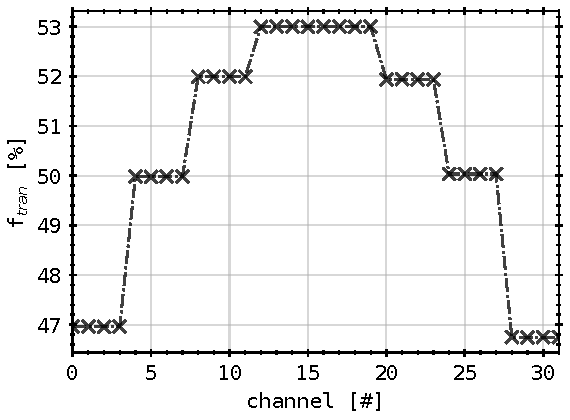
\includegraphics[width=\textwidth]{%
                        content/figures/chapter1/ftran_hbcm.pdf}%
                    \caption{Transmission}\label{fig:ftran}
                \end{subfigure}%
                \caption{\textbf{(a)}: Before and after the ceramic coating treatment and wire mesh installation in front of the detector arrays. Shown are the results of MISTRAL$^{\text{I}}$ tests with and without microwave countermeasures. \textbf{(b)} Transmission factor of wire mesh over channel number. Subsets of detectors are grouped into blocks inside the larger camera array, hence the steps in this curve. Their angle between the lines of sight and mesh normal is equal, yielding the same transmission coefficient.}\label{fig:coating_ftran}%
            \end{figure}%
%
            The previously described absorber, electrical circuit and hardware is capable of acquiring voltages in the range of $\pm$\SI{80}{\milli\volt}, sampled into \SI{16}{bit}, which translates to \SI{2.44}{\micro\volt} acquisition resolution at maximum range. However, this changes in correspondence to the selected acquisition setting, which leads to a minimum resolution of \SI{0.31}{\micro\volt} at $\pm$\SI{10}{\milli\volt} acquisition range. This is also important for the achievable signal-to-noise ratio, where the acquisition range setting defines the smallest possible measurement error by its voltage resolution. The temporal resolution of the ADC is limited by its master clock rate of $f_{master}=\,$\SI{4.9152}{\mega\hertz}. However, the latency of the field programmable gate array (FPGA) inside the ADC, depending on the operation of read and write, ranges between \SIrange{10}{100}{\nano\second}. This is a small perturbation compared to the physical limits of the detector, dominated by its cooling time. The sample frequency of the ADC is given by programmable hexa-/decimal values. With 12-bit encoding, translating to $2^{12}=4096$ possibilities of setting, and taking the minimum and maximum sample window length $T\ix{s, min/max}$ into account, the smallest delta in sample time or frequency becomes%
%
            \begin{align}%
                \Delta T_{sample}=\frac{T_{s, max}-T_{s, min}}{4096}=\text{\SI{0.0095}{\milli\second}}\,,\quad\Delta f_{sample}=\text{\SI{0.0254}{\kilo\hertz}}\,.\nonumber%
            \end{align}%
%
            
            Data acquisition was possible for sample times of $\{0.8, 1.6, 3.2, 6.4, 12.8\}$\SI{}{\milli\second}. One should note that the ADC is capable of operating at another measurement mode, where the acquisition range is sampled twice per cycle period with alternating parity, i.e. between alternating pins resulting in a change of sign, which comes at the benefit of a much smaller signal-to-noise ratio. A further characterisation of this acquisition mode has not been pursued.\\%
            In measurement mode it was found that the noise background caused by small fluctuations in situations without incident radiation is in the range of \SIrange{0.5}{6}{\micro\volt}. This results in a signal-to-noise ratio in high radiation scenarios of at least:%
%
            \begin{align}%
                \begin{split}\label{eq:median_sigma}%
                    \overline{\Delta U}&=\underset{t_{1},t_{2}}{\text{median}}\left(\Delta U\left(t\right)\right)\qquad\qquad\qquad\,\,\,,\,T\ix{start}<t_{1}<t_{2}<T\ix{stop}\\%
                    \sigma_{\Delta U}&=\sqrt{\int_{t_{0}}^{t_{0}^\prime}\left(\Delta U-\overline{\Delta U}\left(t_{0},t_{0}^\prime\right)\right)^2\diff x}\quad\,\,,\,t_{0}<t_{0}^\prime<T\ix{stop}%
                \end{split}\\%
                \text{SNR}&=\frac{\overline{\Delta U}}{\sigma_{\Delta U}}=1000\,\,\widehat{=}\,\,10\lg\left(\frac{\overline{\Delta U}}{\sigma_{\Delta U}}\right)\,\text{dB}=30\,\text{dB}\,.\nonumber%
            \end{align}%
%
            Here, $\overline{\Delta U}$ is the median value in the interval $\left(t_{1},t_{2}\right)$ and $\sigma_{\Delta U}$ the standard deviation. However, they are both calculated at different times: $\sigma_{\Delta U}$ describes the noise before the experiment, while $\overline{\Delta U}$ represents the median of the signal during the discharge. This avoids possibly accounting for plasma radiation fluctuations to contribute to $\sigma_{\Delta U}$.\\%
            The quality of the acquired signal and calibration results have been closely monitored throughout the past, and especially the last experimental campaign. Combined they yield information about the absorber condition and wear or possible discrepancies with the connected electronics. The results can be seen in \cref{fig:opstatistics1} and \cref{fig:opstatistics2}. Shown there is the 99th percentile of both the calibration values and acquisition properties for each main detector across the last experimental campaign. The core bolometry system with its 61 functional detectors successfully participated in 1182 experiment programs.\\%
%
            \begin{figure}[t]%
                \centering%
                \begin{subfigure}{0.48\textwidth}%
                    \includegraphics[width=\textwidth]{%
                        content/figures/chapter1/Rohm_99th_OP12b.pdf}%
                    \caption{Resistance}\label{fig:stat_resistance}%
                \end{subfigure}%
                \hfill%
                \begin{subfigure}{0.48\textwidth}%
                    \includegraphics[width=\textwidth]{%
                        content/figures/chapter1/Kappam_99th_OP12b.pdf}%
                    \caption{Heat capacity}\label{fig:stat_heatcapacity}%
                \end{subfigure}%
                \\%
                \begin{subfigure}{0.48\textwidth}%
                    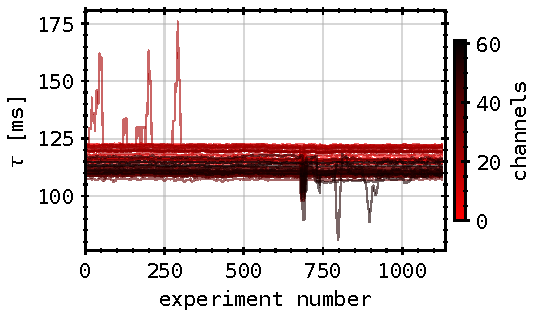
\includegraphics[width=\textwidth]{%
                        content/figures/chapter1/Taum_99th_OP12b.pdf}%
                    \caption{Cooling time}\label{fig:stat_coolingtime}%
                \end{subfigure}%
                \hfill%
                \begin{subfigure}{0.48\textwidth}%
                    \includegraphics[width=\textwidth]{%
                        content/figures/chapter1/abs_offs_99th_OP12b.pdf}%
                    \caption{Offset}\label{fig:stat_offset}%
                \end{subfigure}%
                \caption{Calibration parameters of the core bolometry system at W7-X during OP1.2b. \textbf{(a)} Resistance of the absorber as calculated by \cref{eq:resistance}. \textbf{(b)} Normalized heat capacity of the detector from \cref{eq:heatcapacity}. \textbf{(c)} Cooling time from exponential decay fit to an ohmic heating stage as depicted in \cref{fig:ohmicheating}. \textbf{(d)} Absolute offset in acquisition before the discharge begins.}\label{fig:opstatistics1}%
            \end{figure}%
%
            \autoref{fig:opstatistics1} presents the calibration results of the measurement absorbers, including the resistance, normalized heat capacity, cooling time and signal voltage offset without plasma. The results of \cref{eq:resistance} in \cref{fig:stat_resistance} show very small deviation over time. Plateaus in $R$ indicate individual experiment days, where in-between the camera array temperature slightly deviated. Towards the end of the campaign however three detectors of the vertical bolometer camera particularly diverge, indicating either deterioration or electronic problems. Solving \cref{eq:heatcapacity} for calibrations during OP1.2b yields \cref{fig:stat_heatcapacity}. Similarly, the characteristics of each detector vary only slightly for each experiment. One absorber produces values that greatly diverge from its campaign average within the first ca. 350 experiments. This is likely due to systematic errors in the calibration process or algorithm, since those perturbations no longer appear after. At around experiment number 350 an entire session of about 30 experiments shows collectively smaller heat capacities, which again points to an issue with the first ohmic heating stage during the calibration process or interference of the camera array temperature. Similar results are found for the cooling time data shown in \cref{fig:stat_coolingtime}. The perturbations responsible for the valleys in the heat capacity data however have a reciprocal effect and lead to peaks in the cooling time. For an experiment session of about 30 discharges the cooling time collectively decreases by about 20\% likely because of the above reasons. \cref{fig:stat_offset} shows the fit results from \cref{eq:drift}, i.e. the absolute offset at the start of the discharge when the absorber has equilibrated after engaging the measurement excitation. Generally the values are below \SIrange{1}{2}{\micro\volt}. In single cases, perturbations in the cameras' water cooling can lead to thermal interference, which produces larger offsets and peaks in \cref{fig:stat_offset}. As previously lined out, at typically \SIrange{10}{20}{\milli\volt} acquisition range at \SI{16}{\bit} resolution this compares to the possible minimum \SIrange{0.15}{0.3}{\micro\volt} bit-noise.\\%
%
            \begin{figure}[t]%
                \begin{subfigure}{0.48\textwidth}%
                    \includegraphics[width=\textwidth]{%
                        content/figures/chapter1/std_dev_99th_OP12b.pdf}%
                    \caption{Standard deviation}\label{fig:stat_stddev}%
                \end{subfigure}%
                \hfill%
                \begin{subfigure}{0.48\textwidth}%
                    \includegraphics[width=\textwidth]{%
                        content/figures/chapter1/slope_99th_OP12b.pdf}%
                    \caption{Temperature drift}\label{fig:stat_drift}%
                \end{subfigure}%
                \\%
                \begin{subfigure}{0.48\textwidth}%
                    \includegraphics[width=\textwidth]{%
                        content/figures/chapter1/adj_median_99th_OP12b.pdf}%
                    \caption{Median}\label{fig:stat_median}%
                \end{subfigure}%
                \hfill%
                \begin{subfigure}{0.48\textwidth}%
                    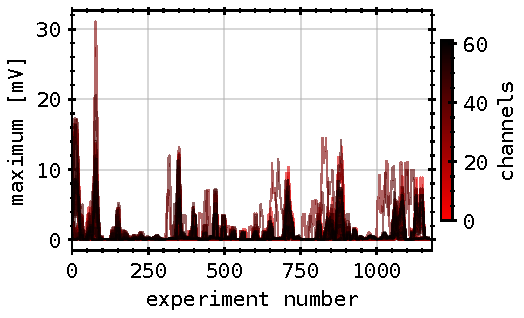
\includegraphics[width=\textwidth]{%
                        content/figures/chapter1/adj_max_99th_OP12b.pdf}%
                    \caption{Maximum}\label{fig:stat_maximum}%
                \end{subfigure}%
                \caption{Operational performance numbers of the core bolometry system at W7-X during OP1.2b. (Top Left) Standard deviation from measurements without plasma background, i.e. 100 samples before ECRH starts. (Top Right) Thermal signal drift (positive). (Bottom Left) Median of signal during plasma discharges. (Bottom Right) Maximum signal for every experiment.}\label{fig:opstatistics2}%
            \end{figure}%
%
            \autoref{fig:opstatistics2} presents the acquisition performance, including the standard deviation, i.e. noise, temperature drift, signal median and voltage maximum. The results of \cref{eq:median_sigma} in \cref{fig:stat_stddev} and \cref{fig:stat_median} portray similar behaviour like the voltage offset in \cref{fig:stat_offset}. Generally, both signal noise and drift are low, predictably in the range of \SIrange{0.5}{1}{\micro\volt} and \SIrange{0.1}{0.5}{\micro\volt\per\second} respectively. This level of noise is around twofold the minimum possible voltage resolution, while the thermal interference drift is even smaller. However, assuming a total acquisition time of \SI{10}{\second}, which was a common requirement during the last experimental campaign, this leads to a baseline offset of up to \SI{50}{\micro\volt} towards the end of the measurement. Longer acquisition times lead to greater perturbations, though their correction remains accessible through the simple fit method in \cref{eq:drift}. In cases where the thermal load onto the absorber or camera device is increased, this value can change significantly as depicted in the first half of the plot, where individual detectors exhibit spikes of up to \SI{2}{\micro\volt\per\second}, which is almost ten times as much as the average expected signal drift. The background noise in \cref{fig:stat_stddev} is largely consistent throughout the past experimental campaign, with collective peaks across multiple tens of experiments, where $\sigma_{\Delta U}$ reaches up to \SI{2.5}{\micro\volt}. %
%
            \begin{table}[t]%
                \centering%
                \begin{tabular}{||c|c|c|c|c||}%
                    \hline\rule{0pt}{.75\normalbaselineskip}%
                    property & $\kappa_{M}$ $\left[\text{A}^{2}\right]$ & $R_{M}$ $\left[\right.$\SI{}{\ohm}$\left.\right]$ & $\tau_{M}$ $\left[\text{ms}\right]$ & $V\ix{off}$ $\left[\right.$\SI{}{\micro\volt}$\left.\right]$ \\[.5ex]\hline\hline%
                    median & $0.724$ & $0.987$ & $110.57$ & $0.204$ \\\hline%
                    deviation & $0.0545$ & $0.011$ & $4.93$ & $31.11$ \\[.5ex]\hline%
                \end{tabular}%
                \\[1ex]%
                \begin{tabular}{||c|c|c|c|c||}%
                    \hline\rule{0pt}{.75\normalbaselineskip}%
                    property & $\sigma_{\Delta U}$ $\left[\right.$\SI{}{\micro\volt}$\left.\right]$ & $V\ix{drift}$ $\left[\right.$\SI{}{\micro\volt\per\second}$\left.\right]$ & $\overline{\Delta U}$ $\left[\text{mV}\right]$ & maximum $\left[\text{mV}\right]$ \\[.5ex]\hline\hline%
                    median & $0.339$ & $0.057$ & $0.042$ & $1.186$ \\\hline%
                    deviation & $12.586$ & $27.621$ & $0.032$ & $3.704$ \\[.5ex]\hline%
                \end{tabular}%
                \vspace*{0.5cm}%
                \caption{Median and standard deviation of all previously discussed properties of the calibration and acquisition. Results taken from \cref{fig:opstatistics1} and \cref{fig:opstatistics2}.}\label{tab:stat_numbers}%
            \end{table}%
%
            Those peaks extend past one single event, which means they are not linked to experimental circumstances, but revert and flatten out, indicating that they are reversible and not connected to absorber conditions. This is most likely due to issues with the excitation voltage of the Wheatstone bridge by perturbations in the electrical power supply of the diagnostic. \autoref{fig:stat_median} displays results from \cref{eq:median_sigma}, which tries to establish an average gain of the detector signal across OP1.2b. This shows that the expected signal from plasma and stray microwave radiation, as well as thermal perturbation is at least two orders of magnitude larger than the previously discussed drift and noise, and one greater than the average offset. The last \cref{fig:stat_maximum} establishes the maximum signal per experiment. Values above \SI{10}{\milli\volt} repeatedly occur across multiple sessions, i.e. beyond a set of tens of discharges, indicating high performance and high radiation scenarios. This also solidifies the decision to set the range of acquisition to \SIrange{10}{20}{\milli\volt}, depending on the geometric location of the channel - a channel monitoring the scrap-off layer likely yields smaller signals, and therefore performs better at high resolutions or smaller ranges -, so high radiation scenarios are measured adequately.\\%
%
            \begin{table}[t]%
                \centering%
                \begin{tabular}{||c|c|c|c|c|c|c||}%
                    \hline\rule{0pt}{.75\normalbaselineskip}%
                    property $x$ & $\Delta U$ & $\diff \left(\Delta U\right)/\diff t$ & $\diff t$ & $U_{0}$ & $R\ix{L}$ & $f\ix{bridge}$ \\[.5ex]\hline\hline%
                    value $s_{x}$ & \SI{0.5}{\micro\volt} & \SI{1}{\micro\volt\per\second} & \SI{15}{\micro\second} & \SI{1}{\milli\volt} & \SI{1}{\milli\ohm} & \SI{1}{\hertz} \\[.5ex]\hline%
                \end{tabular}%
                \\[1ex]%
                \begin{tabular}{||c|c|c|c|c||}%
                    \hline\rule{0pt}{.75\normalbaselineskip}%
                    property $x$ & $C\ix{C}$ & $\Delta I\left(0\right)$ & $\Delta I\left(\infty\right)$ & $R\ix{C}$ \\[.5ex]\hline\hline%
                    value $s_{x}$ & \SI{0.5}{\nano\farad} & \SI{1}{\micro\ampere} & \SI{1}{\micro\ampere} & \SI{1}{\milli\ohm} \\[.5ex]\hline%
                \end{tabular}%
                \vspace*{0.5cm}%
                \caption{Systematic errors and standard deviation of measurement properties that contribute to the bolometer equation \cref{eq:bolometer_adv}.}\label{tab:gauss}%
            \end{table}%
%
            The previously shown results from \cref{fig:opstatistics1} and \cref{fig:opstatistics1} have been compiled in \cref{tab:stat_numbers}. Median values are representative of the discussed quality of the calibration process and acquisition. Their standard deviations are a measure to the consistency of the performance, while also indicating how exceptional circumstances, e.g. environmental changes can significantly alter, if not corrupt the measurement results.\\%
            Besides analysing the measurement data over a longer period, one can also find an analytical approach to the measurement error. Based on bolometer \cref{eq:bolometer_adv} the \textit{Gaussian\footnote[1]{Johann Carl Friedrich Gauss *~Apr. 30, 1777 \textdagger~Feb. 23, 1855} error propagation} or \textit{propagation of uncertainty} can be calculated using the values from \cref{tab:gauss} and the equation for variance of an analytical function with independent variables. Let $s_{x_{j}}$ be either the standard deviation, if available, or systematic error of variable $x_{j}$. Therefore, the systematic error of $P\ix{M}$ the power onto the absorber becomes:%
%
            \begin{align}%
                s_{P_{M}}^{2}=\sum_{j}\left(\frac{\partial P_{M}}{\partial x_{j}}\right)^{2}s_{x_{j}}^{2}=1.599\,\text{µW}\label{eq:gaussian}%
            \end{align}%
%
            This error is small, especially when compared to common measurement values of >\SI{0.1}{\milli\watt}. Similarly, this characterisation supports the previous findings of small noise levels or large signal-to-noise ratios.\\%
            \newline%
            Generally, given a constant background pressure and temperature of the camera, the W7-X bolometer diagnostic performs well within the required specifications, while featuring a high signal-to-noise ratio $\text{SNR}>1000$ at high temporal resolution for this type of sensor. Results that will later be discussed in this work are within those measurement specifications and have been cleared for consistency.%
%
    \section{Plasma Radiation Power}\label{sec:rad_powerloss}%
%
        % Plasma power balance.%
        The goal of the bolometer system at W7-X is to measure the spatial and temporal evolution of the irradiated power from the plasma within its field of view. Ultimately, the bolometer is used to provide a totally calibrated global plasma radiation power loss and the underlying local emissivity. The provided information are critical towards the protection of the machine and experiment control, with regard to plasma profiles and instabilities\cite{Zhang2010,Grulke2018}. In particular, the bolometer measurements are necessary to understand  energy loss processes and transport, since the majority of the radiation power is expected to come from intrinsic impurities\cite{Zhang2014,Zhang2019}. This, in turn, is important towards the assessment of the energy confinement quality and performance of the plasma\cite{Fuchert2018}. The tomographic inversion of the line-integrated channel signals can be used to investigate the diffusion and transport of the plasma as well as the impurities\cite{Murari2007}. However, the most important task of the bolometer is to provide the radiation power from the plasma, since large radiation losses reduce the in part convective thermal loads on target components and dissipate them into \SI[parse-numbers=false]{4\pi}{\steradian}, which is highly relevant for the lifetime of the machine and its safety\cite{Arnoux2011}.\\%
        Following will be an introduction to the methodology of calculating the global radiation power and local emissivity, i.e. a total radiation power loss from the plasma in \cref{subsec:global} and a radially or two-dimensionally resolved power density at the given field of view of the camera system in \cref{subsec:local}.
%
        \subsection{Global}\label{subsec:global}
%
        % Global power balance.%
            The line of sight geometry has been thoroughly introduced and established in detail previously in \cref{subsec:losgeometry}. \autoref{fig:los_vessel} shows the conceptional setup of the lines of sight inside the vessel. An understanding of the geometry and transmissivity of the detector-aperture lines of sight are crucial to the development of a global radiation power measurement. The estimation of the global radiative power loss from the plasma will be based on geometric calculations of the individual detectors lines of sight and assumptions about the irradiating plasma volume.\\%
            Previously, the total incident power onto a single detector $P_{M}$ has been established in \cref{eq:bolometer_adv}. Given calibration results for the resistance, cooling time and heat capacity one can thereby calculate the total power for each camera $C$ by their respective detector numbers $M\in S_{C}$. In order to extrapolate the radiation power measured in the bolometer plane of W7-X to the entire torus one needs to account for the difference in volume and therefore make assumptions about the emissivity distribution along the magnetic field lines. Let the total irradiating plasma volume to be $V\ix{P, tor}$. A schematic of the radiation domain can be seen in \cref{fig:domain_schematic}, where the magnetically confined region and island chain is fully covered. In agreement to Peterson and Zhang et al.\cite{Peterson2016_EPS,Zhang2013}, three-dimensional EMC3\footnote[1]{EMC3: Edge Monte Carlo 3D; plasma transport simulations in island divertors}-EIRENE\footnote[2]{EIRENE: neutral gas transport Monte Carlo code} Monte Carlo plasma transport simulations of the scrape-off layer (SOL)\cite{Feng1997,Reiter2005} indicate that the irradiating volume extends as far as $r\ix{eff}=1.35\,r\ix{a}$, the minor (effective) plasma radius from the magnetic axis. Simulations focussing on the intrinsic impurities carbon and oxygen at different heating powers and radiation fractions $f\ix{rad}=0.4-0.9$ - the ratio of total radiation power loss and input (heating) power $P\ix{H}$ - show a total plasma volume of $r\ix{eff}^{2}/r\ix{a}^{2}=1.82\mathrel{\hat{=}}182\%$ of $V\ix{LCFS}$, the volume of the last closed magnetic flux surface.%
%
            \begin{align}%
                f\ix{rad}=\frac{P\ix{rad}}{P\ix{H}}\label{eq:fraction}%
            \end{align}%
%
            By design, a domain of effective radius $1.3\,r\ix{a}$ is necessary to accommodate all lines of sight of the bolometer system adequately inside the vessel, since smaller volumetric projections do not intersect with the line of sight of the outermost channels of the cameras. Assuming the predictive quality of these calculations to be adequate, EMC3 simulations should be performed for all magnetic configurations, experiment scenarios and machine conditions to find the corresponding irradiating plasma volume. However, this in itself is a very taxing and computationally expensive task and therefore outside the scope of this work. Ideally, the lines of sight of the bolometer cover the whole plasma domain so that the outermost channels yield $P\ix{M}\approx 0$, which in contrast will be relevant later on in this work. This is especially important towards boundary conditions of tomographic inversion in \cref{chap:inversions}. The assumption of $V\ix{P, tor}=f\ix{P}V\ix{LCFS}=1.3^2\,V\ix{LCFS}$, where $f\ix{P}$ is the volumetric factor, generally yields good results, which will later be discussed in more detail for the performance of the tomographic inversion in \cref{sec:expdata}. On should note here that $f\ix{P}$ is effectively a scaling factor towards the total radiated power loss of the plasma.\\%
%
            \begin{figure}[t]%
                \centering%
                \begin{subfigure}{0.43\textwidth}%
                    \includegraphics[width=\textwidth]{%
                        content/figures/chapter1/los_example_polygon.pdf}%
                    \caption{Line of sight volume}\label{fig:los_volume_example}%
                \end{subfigure}%
                \hspace*{1.0cm}%\hfill%
                \begin{subfigure}{0.52\textwidth}%
                    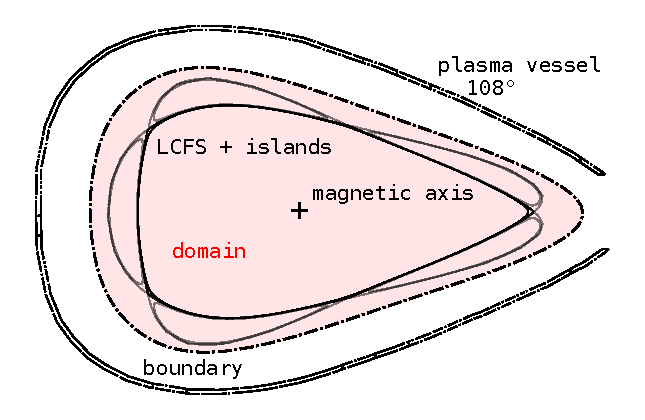
\includegraphics[width=\textwidth]{%
                        content/figures/chapter1/vessel_lcfs_domain.pdf}%
                    \caption{Bolometer plane}\label{fig:domain_schematic}%
                \end{subfigure}%
                \caption{\textbf{(a)}: Trapezoidal LOS cone through an exemplary volume element. The blue lines indicate the intersection of the line of sight and domain, i.e. test cube. Marked red is the length of the center LOS inside the volume. \textbf{(b)}: A schematic assembly of the plasma vessel at 108° toroidally with outlines of the LCFS and attached $5/5$-island chain from an exemplary Poincaré  map. The estimation domain is marked with the dot-dashed line and red fill pattern. Approximately this equals 169\% of the surface area/volume of the LCFS.}\label{fig:torus_domain}%
            \end{figure}%
%
            As indicated in \cref{subsec:losgeometry}, some parts of the detectors are only partially exposed to plasma radiation by the aperture. Hence, one has to establish a relation between the line integral through $V\ix{P, tor}$ and geometry of detector and aperture to find the plasma radiation along the line of sight. Let $P_{\text{rad}, M}$ be the average plasma radiation along the line of sight of detector $M$.%
%
            \begin{align}%
                P_{\text{rad}, M}=\iiint \frac{g\ix{rad}\left(\vec{r}\right)}{\widetilde{K}_{M}\left(\vec{r}\right)}\,\,\diff\vec{r}\label{eq:total_line}
            \end{align}%
%
            In \cref{eq:total_line}, $\widetilde{K}_{M}\left(\vec{r}\right)$ is the etendue of detector $M$ and $g\ix{rad}\left(\vec{r}\right)$ the radiation distribution of the plasma. The transmission function $\widetilde{K}_{M}$ describes how light enters the bolometer and reaches the detector. The measurement of power onto the detector does not distinguish between the parts of the absorber that are hit by radiation. Therefore, the total transmission or etendue no longer is a function of $\vec{r}$ but rather only of detector and aperture geometry, $\widetilde{K}_{M}\left(\vec{r}\right)=\widetilde{K}_{M}$. \autoref{eq:etendue_woline} has already presented the etendue in \cref{subsec:losgeometry}.\\%
            The zero-dimensional measurement of radiation power per detector and point in time includes a geometric simplification about $g\ix{rad}$: one assumes that the radiation is equally distributed along the total line of sight length $L_{M}$. In order to introduce the power onto the detector $P_{M}$ from \cref{eq:bolometer_adv} to \cref{eq:total_line}, we arrive at:%
%
            \begin{align}%
                \iiint g\ix{rad}\left(\vec{r}\right)\,\diff\vec{r}&\overset{!}{=}\frac{P_{\text{bolo}, M}}{L_{M}}\equiv\frac{P_{M}}{L_{M}}\,\,,\nonumber\\%
                K_{M}&=\widetilde{K}_{M}\cdot L_{M}\,\,,\nonumber\\%
                \Rightarrow\quad P_{\text{rad}, M}&=\frac{P_{M}}{K_{M}}\,\,.\label{eq:etendue_power}%
            \end{align}%
%
            Therefore, $P_{\text{rad}, M}$ becomes the radiation distribution (density) along the line of sight of detector $M$. It is also referred to as \textit{chord profile} or \textit{chord brightness}, which will later be introduced more thoroughly in \cref{subsec:local}. The final step towards a global radiation power loss is the extrapolation from the investigated volume of the bolometer camera. Let the line of sight volume of channel $M$ inside the radiation domain be $V_{M}$. An example of how this is defined can be seen in \cref{fig:los_volume_example}. A more detailed description and examples of volumetric calculations can be found in \cref{sec:evalmetrics}. The radiation power in the plane of camera $C$, $P_{\text{rad}, C}$ and therefore total radiation power from the plasma $P\ix{rad}$ can be estimated using:%
%
            \begin{align}%
                V_{C}&=\sum_{M}^{S_{C}}\,V_{M}\nonumber\\%
                \Aboxed{%
                    P\ix{rad}\coloneqq P_{\text{rad}, C}&=\frac{V\ix{P, tor}}{V_{C}}\,\sum_{M}^{S_{C}}\,\frac{P_{M}V_{M}}{K_{M}}\,,\qquad C\in\left(\text{HBC, VBC}\right)%
                }\label{eq:prad_total}%
            \end{align}%
%
            \autoref{eq:prad_total} denotes the total, global radiation power from the plasma as measured by the bolometer. This quantity will usually be introduced as $P\ix{rad}$ generally, or $P\ix{rad, HBC/VBC}$ to specify the camera array that is used to extrapolate from. A set of volumes $V_{M}$ and etendues $K_{M}$ for the magnetic standard configuration with $V\ix{P, tor}=1.3^2\,V\ix{LCFS}$ for all three cameras can be seen in \cref{fig:volume_channels}.\\%
            \autoref{fig:power_prad_ex} shows an example of how the calculations using \cref{eq:bolometer_adv} and \cref{eq:prad_total}, together with values taken from \cref{fig:volume_channels}, contribute to a total radiation power estimation for an experiment in W7-X during the last experimental campaign. The total absorbed power $P_{M}$ onto the detector from the HBC is roughly half of that from the VBC due to the larger distance between detector and pinhole, reducing the radiation intensity per surface area at the cameras' absorber plane. Expectedly, when accounting for the respective etendues and line of sight volumes $P\ix{rad, HBC}$ and $P\ix{rad, VBC}$ represent the same radiative power loss roughly within a 5\% margin of error. However, in highly poloidally asymmetric plasma radiation scenarios this deviation can very strongly. Individual assessments of the local emissivity profiles, which will be discussed further below, or tomographic inversions are necessary to address the radiative power loss adequately in this case.\\%
%
            \begin{figure}[t]%
                \centering%
                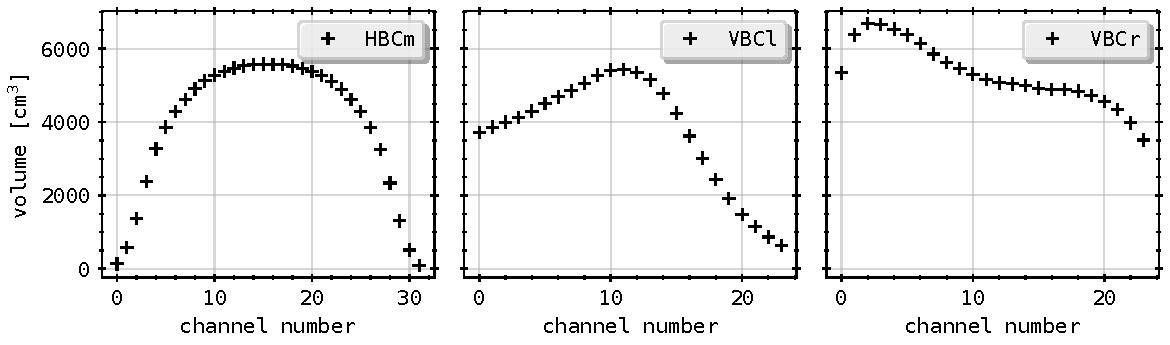
\includegraphics[width=0.95\textwidth]{%
                    content/figures/chapter1/volume_per_camera.pdf}\\%
                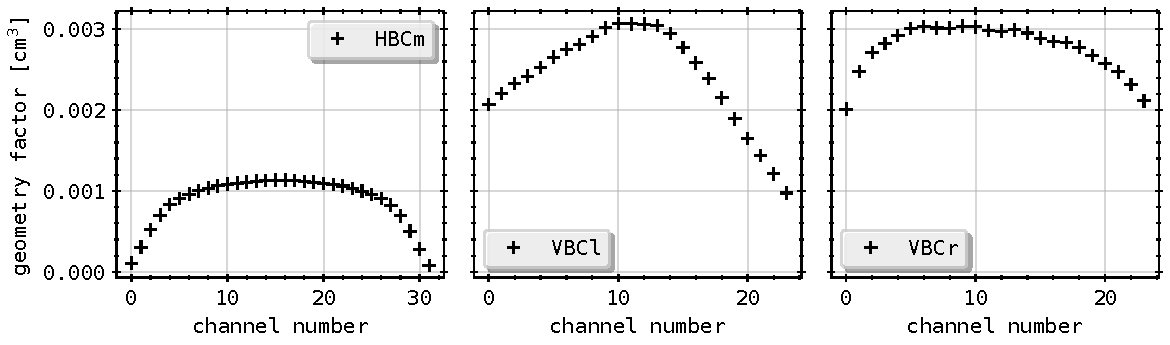
\includegraphics[width=0.95\textwidth]{%
                    content/figures/chapter1/kfac_per_camera.pdf}%
                \caption{Line of sight volumes $V_{M}$ (top) and Etendues $K_{M}$ (bottom) of all camera arrays. Note how the bolometers have been designed in a way that all cameras roughly contribute the same LOS volume, while due to differences in the pinhole design etendues are twice as large for the vertical arrays.}\label{fig:volume_channels}%
            \end{figure}%
%
            Given the consistency of the calibration data, volumetric estimations for the required magnetic configuration and measurement data itself, extrapolations made using \cref{eq:prad_total} have proven fit the radiation level very well when incorporating and comparing to other diagnostics that are used to provide information about the experimental performance. One metric to measure the adequacy of the total radiated power loss by is the \textit{global power balance}. A more detailed discussion of how the accuracy of $P\ix{rad}$ can be addressed will follow further below in \cref{subsec:local} and \cref{subsec:power_balance}. One should also note that a different approach, instead of estimating the irradiation plasma region as $V\ix{P, tor}$ from magnetic equilibrium calculations, is to directly calculate the volume using the boundaries of the radial radiation profile as measured by the bolometer. This will also be discussed in more detail in the next section.%
%
            \begin{figure}[t]%
                \centering%
                \begin{subfigure}{0.47\textwidth}%
                    \includegraphics[width=\textwidth]{%
                        content/figures/chapter1/%
                        power_example_20181010036_HBCm.pdf}%
                \end{subfigure}%
                \begin{subfigure}{0.47\textwidth}%
                    \includegraphics[width=\textwidth]{%
                        content/figures/chapter1/%
                        power_example_20181010036_VBC.pdf}%
                \end{subfigure}\\%
                \hspace*{-0.4cm}%
                \includegraphics[width=0.9\textwidth]{%
                    content/figures/chapter1/%
                    prad_example_20181010036_m_combined.pdf}%
                \caption{%
                    XP20181010.36\\%
                    \textbf{(top)} Absorbed power per channel $P_{M}$ by \cref{eq:bolometer_adv} over time for HBC (left) and VBC (right). \textbf{(bottom)} Total radiative power loss as extrapolated from the above detector measurements using \cref{eq:prad_total}. Example discharge with thermal helium beam density control by interferometry in standard magnetic configuration and \SI{5.72}{\mega\watt} input ECRH power, achieving \SI{1.2e20}{\per\cubic\meter} and \SI{2.5}{\kilo\electronvolt} electron density and temperature, respectively.}\label{fig:power_prad_ex}%
            \end{figure}%
%
        \subsection{Local}\label{subsec:local}%
%
            % Local power.%
            The global radiation power as measured by the bolometer diagnostic has been introduced. In addition to the absolute radiative power loss from the plasma, the local, radially or two-dimensionally resolved emissivity at the given field of view of the bolometer system is just as important in order to understand the impact of plasma impurities and transport on the radiation profile and vice versa.%
%
            \subsubsection*{Chord Brightness Profile}%
%
                Let us assume a plasma with $V\ix{P, tor}=1.3^{2}V\ix{LCFS}$ as shown in \cref{fig:domain_schematic}. This area can be sectioned in both radial and poloidal direction to create a two-dimensional grid in $\vec{r}=\left(r,\,\vartheta\right)$ from the perspective of the magnetic axis, or $\vec{r}=\left(r,\,z,\,\vartheta\right)=\left(r,\,z\right)$, i.e. cylinder coordinates as seen from the center of the machine, where $\varphi=108^{\circ}$ the toroidal angle in the bolometer plane. \autoref{fig:los_grid_emiss} on the left shows how such a grid can potentially be constructed for any magnetic configuration. As the domain boundary is modelled after the last closed flux surface of that magnetic configuration, the width of those $N\ix{r}$ radial sections is coupled to the minor plasma radius $r\ix{a}$, e.g. $\diff r=1.3\,r\ix{a}\,/\,N\ix{r}$ for a $1.3^{2}V\ix{LCFS}$ domain. Likewise, the $N_{\vartheta}$ poloidal cross-sections are calculated from the full $2\pi$ angle, $\diff\vartheta=2\pi/N_{\vartheta}$. A common setting would be $N\ix{r}=20$ and $N_{\vartheta}=150$. This method will also be used later for geometric calculations towards tomographic inversions in \cref{chap:inversions}. One should note that increasing both radial and poloidal (and/or toroidal) step counts may introduce numerical artefacts due to overfitting during tomographic inversions of the line integrated measurements.\\%
                With \cref{eq:etendue_woline} the concept of infinitesimal detector and aperture subdivisions has been introduced. Let us rewrite the integral over both the detector and aperture as a single integral over differential etendues, i.e:%
%
                \begin{align}%
                    \iint_{A, M}\frac{\cos\left(\alpha\right)\cos\left(\beta\right)}{2\pi d^{2}}\diff A_{M}\diff A_{A}\overset{!}{=}\int_{M}\diff \widetilde{K}_{M}\,\,.\label{eq:diff_etendues}%
                \end{align}%
%
                In order to assess the radiation distribution in the plane of the bolometer cameras one has to know where the line of sight cone is located in three-dimensional space. Therefore, the grid in \cref{fig:los_grid_emiss} has to be extended in toroidal direction for $\pm 2.5^{\circ}$ to account for the respective tilt of the camera and the width of the line of sight cones. This is done by repeating the same approach as before for flux surfaces of the same magnetic configuration at corresponding toroidal locations. One should note that the grid in this figure is not exactly only constructed from segmented magnetic flux surfaces calculations. This is in fact the projection of the enclosing meshes onto the actual bolometer camera plane, which one remembers to be significantly tilted in toroidal direction. Practically, the pixel corners have been traced in direction of the torus from one VMEC equilibrium to the next. The potential intersections of those lines with the bolometer plane are calculated and constructed into the presented grid. If not stated otherwise, this will be the case for all two-dimensional meshes in the triangular plane from here on.\\%
%
                \begin{figure}[t]%
                    \centering%
                    \includegraphics[width=0.9\textwidth]{%
                        content/figures/chapter1/%
                        vessel_combinedL_poincare.pdf}%
                    \caption{\textbf{(left)}: Standard magnetic configuration based grid with 20 radial and 150 poloidal divisions that covers $1.3^2\,V\ix{LCFS}$. Marked are the center position of the individual apertures (black crosses) for all cameras. For reference one line of sight cone (noted in electrical channel number) per camera array has been included. \textbf{(right)}: Total geometry contribution per pixel summed up from all three camera arrays.}\label{fig:los_grid_emiss}%
                \end{figure}%
%
                Let us assume a voxel $v^{\left(i,j,k\right)}$, i.e. a six sided polyeder with eight corners made up out of neighbouring grid intersections. The pixels $p^{\left(i,j\right)}$ in \cref{fig:los_grid_emiss} are achieved by collapsing, i.e. summation of all voxels at index $\left(i,j\right)$ for all $N_{\vartheta}$ toroidal divisions. Let $T^{\left(i,j\right)}_{M}$ be the geometrical contribution, i.e. local sensitivity of the bolometer absorber $M$ to radiation for pixel $p^{\left(i,\,j\right)}$. With $L^{\left(i,j,k\right)}_{M}$ the line of sight section length from differential $\diff A_{M}$ through $\diff A_{A}$ (see \cref{eq:diff_etendues}) inside the voxel $v^{\left(i,\,j,\,k\right)}$, the geometrical contribution becomes:%
%
                \begin{empheq}[box=\fbox]{align}%
                    T^{\left(i,j\right)}_{M}=\sum_{k=1}^{N_{\vartheta}}T^{\left(i,j,k\right)}_{M}=&\sum_{k=1}^{N_{\vartheta}}\left(\int_{M}L^{\left(i,j,k\right)}_{M}\diff\widetilde{K}_{M}\right)\label{eq:emissivity}\\%
                    T^{\left(i,j,k\right)}_{M}=&\left\{%
                    \begin{array}{ll}%
                        0&,\,\,M\text{ not in }v^{\left(i,j,k\right)}\\%
                        L^{\left(i,j,k\right)}_{M}\diff\widetilde{K}_{M}&,\,\,\text{else}%
                    \end{array}\right.\nonumber%
                \end{empheq}
%
                The geometrical contribution can be interpreted as the convolution of etendue and line of sight length at a given position. It describes the impact radiation at this location yields onto the absorber. The sum of all camera emissivities can be found in \cref{fig:los_grid_emiss}. The etendue $\widetilde{K}_{M}$ is contributing to $T^{\left(i,j\right)}_{M}$, which again is calculated from the relative camera aperture and detector geometry. For the VBC, the etendues are roughly two times larger than those of the HBC, as seen in \cref{fig:volume_channels}, which, in turn, also yields larger $T^{\left(i,j\right)}$. Additionally, both VBC array lines of sight overlap close to their respective apertures, thus further increasing the \textit{local sensitivity} in front of the vertical camera relative to its horizontal counterpart.\\%
%
                \begin{figure}[t]%
                    \centering%
                    \includegraphics[width=\textwidth]{%
                        content/figures/chapter1/%
                        reffLoS_minEmiss_normalized.pdf}%
                    \caption{Normalized effective plasma radius $r\ix{eff}$ in units of the minor plasma radius $r\ix{a}$=\SI{0.539}{\meter} along the line of sight of each detector and camera array. Both methods from \cref{eq:effective_radM}(a) and (b) are shown as 'min' and '$\varepsilon$', respectively.}\label{fig:refflos}%
                \end{figure}%
%
                \autoref{eq:emissivity} can be used to quantitatively describe the position of the line of sight of detector $M$ in two-dimensional space for one toroidal position by attributing each an effective plasma radius $r_{\text{eff}, M}$. From magnetic equilibrium calculations, on which the grid around the magnetic axis $\vec{r}\ix{mag}=\left(r\ix{mag}, z\ix{mag}\right)$ is based, every pixel $p^{\left(i,\,j\right)}$ is given a $r\ix{eff}^{\left(i,j\right)}$ for their center position $\vec{p}_{0}^{\,\left(i,j\right)}=\left(r_{0}^{\left(i,j\right)}, z_{0}^{\left(i,j\right)}\right)$. The effective plasma radius of the line of sight of detector $M$ can be written as:%
%
                \begin{align}%
                    &r_{\text{eff}, M}=\left\{%
                    \begin{array}{ll}%
                        \underset{T^{\left(i,j\right)}_{M}>0}{\text{argmin}}\,\left(r\ix{eff}^{\left(i,j\right)}\right)&\quad\text{(a)}\\%
                        \,\\%
                        \displaystyle\sum_{i=0}^{N_{r}}\sum_{j=0}^{N_{\vartheta}}\left(T_{M}^{\left(i.j\right)}\,r\ix{eff}^{\left(i,j\right)}/\sum_{i=0}^{N_{r}}\sum_{j=0}^{N_{\vartheta}}T_{M}^{\left(i,j\right)}\right)&\quad\text{(b)}%
                    \end{array}\right.\label{eq:effective_radM}\\%
                    &\quad\text{sgn}\left(r\ix{eff}^{\left(i,j\right)}\right)=\left\{%
                    \begin{array}{ll}%
                        -1,&\left(z_{0}^{\left(i,j\right)}<z\ix{mag}\vee M\in S\ix{HBC}\right)\wedge\\%
                        &\,\,\,\,\left(r_{0}^{\left(i,j\right)}<r\ix{mag}\vee\left(M\in S\ix{VBCl}\vee M\in S\ix{VBCr}\right)\right)\\%
                        +1,&\text{else}%
                    \end{array}\right.\nonumber%
                \end{align}%
%
                \autoref{eq:effective_radM}(a) and (b) introduce an effective plasma radius for every detector. Method (a) returns the minimum radius along the line of sight of detector $M$, while method (b) calculates the effective radius by weighting the individual contributions $r\ix{eff}^{\left(i,j\right)}$ with their respective, normalized $T_{M}^{\left(i,j\right)}$. The sign convention in $\text{sgn}\left(r\ix{eff}^{\left(i,j\right)}\right)$ is used to distinguish between outboard/upside and inboard/downside lines of sight. The normalization of both \cref{eq:effective_radM}:(a) and (b) to the magnetic standard configurations minor plasma radius $r\ix{a}$ can be found in \cref{fig:refflos}. If not stated otherwise, going forward projection method \cref{eq:reffective_radM}:(a) is used whenever radial profiles of bolometer measurements are presented.\\%
                \autoref{eq:effective_radM}(a) yields a nearly linear spectrum of radii up until the upper- and lowermost channels of the HBC, where the line of sights only graze the outer pixels. Qualitatively, \cref{eq:effective_radM}(b) yields similar results, as the effective radius is decreasing monotonous for all camera arrays. However, by weighting the individual contributions with their local sensitivity, $r_{\text{eff}, M}$ represents the radial position which the respective detector $M$ is the most sensitive to. Although all cameras have detectors covering the center of the plasma and magnetic axis (see \cref{fig:los_vessel}), results of \cref{eq:effective_radM}(b) in \cref{fig:refflos} do not support this. Disentangling the convolution of line integrated measurements and locally varying emissivities, in order to assess the radiation distribution, therefore poses a great challenge. The simplest representation of the local radiation distribution is given by the chord profile:%
%
                \begin{empheq}[box=\fbox]{align}%
                    P_{\text{chord}, M}\coloneqq P_{\text{rad},M}\mathrel{\hat{=}}\frac{P_{M}}{\displaystyle\int_{M}L_{M}\,\diff\widetilde{K}_{M}}\overset{!}{=}\frac{P_{M}}{\sum_{i=0}^{N_{r}}\sum_{j=0}^{N_{\vartheta}}\sum_{k=0}^{N_{\varphi}}T\ix{M}^{\left(i,j,k\right)}}\,\,.\label{eq:chord_profile}%
                \end{empheq}%
%
                The chord profile $P_{\text{chord}, M}$ describes the average power per volume or average brightness along the line of sight of detector $M$. Combined results of \cref{eq:effective_radM}(a) and \cref{eq:chord_profile} can be found in \cref{fig:chord_examples}. The top figure shows the combined profiles of all cameras for one point in time. The HBC covers the entire volume, whereas a selection of detectors from both vertical arrays link together for a slightly decreased coverage. The included error bars are barely visible for channels with a significant SNR, i.e. $r_{\text{eff}, M}\in\left(-1.0, 1.0\right)$. Greater uncertainties occur where the SNR is significantly smaller. One should also note that on the positive end of the horizontal camera profile, one channel reports negative values, indicating issues with offset and noise characterisation. The line integrated measurements of all cameras are generally in agreement, with congruence within the last closed flux surface and small differences around the separatrix. This is, however, rather an exception than the rule and will be discussed in more detail in \cref{sec:drawbacks} and \cref{sec:expdata}. The temporal profile evolutions in the bottom figure show a rapid inwards transition of plasma radiation between \SIrange{3.1}{3.35}{\second}. Similarly to the above, profiles for all times from the HBC and VBC indicate radiation mainly from the plasma edges, with decreased intensity in the core of the discharge and a steep drop-off outwards. The profiles of the horizontal camera and right vertical array are not symmetric around the magnetic axis, i.e. $r\ix{eff}=0$. They show a small radial displacement towards the lower, inboard side of the plasma, i.e. $r\ix{eff}<0$ or $z<z\ix{mag}$ and $r<r\ix{mag}$ - $r\ix{max}$ and $z\ix{max}$ being the toroidal radius and height of the magnetic axis.\\%
%
                \begin{figure}%[t]
                    \centering%
                    \includegraphics[width=.7\textwidth]{%
                        content/figures/chapter1/chord_example.pdf}\\%
                    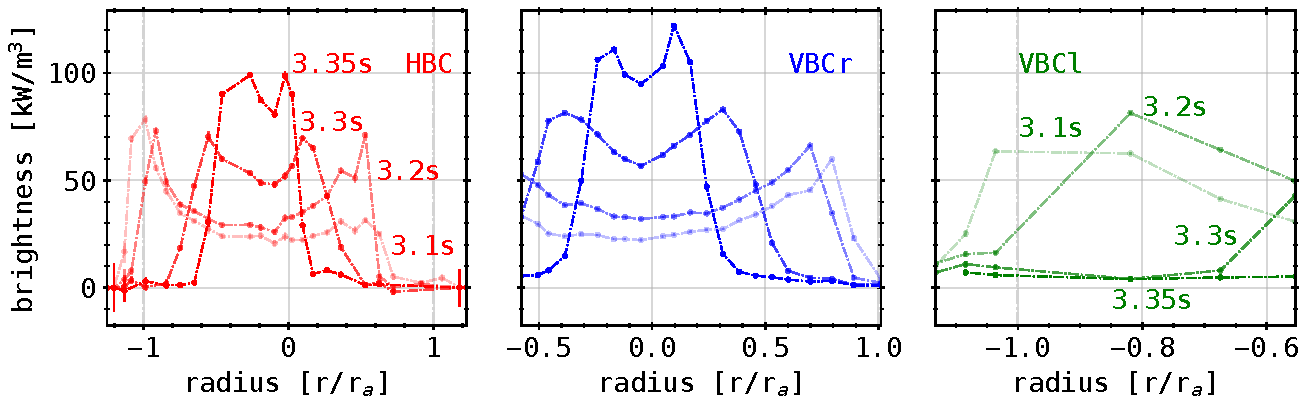
\includegraphics[width=.8\textwidth]{%
                        content/figures/chapter1/chord_example_evolution.pdf}%
                    \caption{%
                        XP20180725.44\\%
                        Example chord brightness profiles for \cref{eq:chord_profile} at \textbf{(top)} \SI{3.0}{\second} and \textbf{(bottom)} a temporal evolution between \SIrange{3.1}{3.35}{\second}. Plot abscissa is given by the minor plasma radius normalization of \cref{eq:effective_radM}(b). The location of the last closed flux surface at 1.0 (-1.0 respectively) has been marked. This discharge was performed in a high magnetic mirror configuration at \SI{1.3}{\mega\watt} ECRH power.}\label{fig:chord_examples}%
                \end{figure}%
%
                The chord brightness represents a convoluted radial radiation profile that can yield information on plasma asymmetry and power loss. Under certain assumptions the chord profile can also indicate dominant impurities that contribute to the cooling of the plasma. For more reference see \cref{sec:strahlmodel}.
%
            \subsubsection*{Radial Profile and Tomography}%
%
                With the multichannel, multicamera bolometer system at Wendelstein 7-X the line integrated measurements can be used to perform tomographic inversions in order to obtain two-dimensional radiation distributions in one plane of the device. Tomographic reconstructions are generally used to solve multidimensional geometric problems of inversion to find solutions for a system with a finite number of projections. Different mathematical models exist in order to invert the line integrals of the projections. In the case of the two-camera W7-X bolometer system in the triangular shaped plane, the number of free parameters, represented by the total number of pixels, is far greater than the number of constraints, i.e. the line of sight intersections. Such an \textit{ill-posed}, or \textit{under-constrained} problem is difficult to solve and requires mathematical effort and \textit{a priori} information or assumptions about the potential profile.\\%
                For simplification, assume the measurement system and distribution profile to be in one plane of $\left(x,\,y\right)$. Let $r$ be the distance to the coordinate center and $\vartheta$ the enclosed angle between $\vec{r}=\left(x,\,y\right)$ and $\vec{e}_{x}$ the unit vector in $x$ direction. Also, let $f\left(x\,,y\right)$ be an unknown distribution. The line integral along $L$ and its parametrisation with $x\left(t\right)=t\sin\left(\vartheta\right)+r\cos\left(\vartheta\right)$ and $y\left(t\right)=-t\cos\left(\vartheta\right)+r\sin\left(\vartheta\right)$ are used in:%
%
                \begin{align}%
                    \begin{split}\label{eq:radon_transform}%
                        \mathcal{R}\,f_{L}&=\int_{L}f\left(x,y\right)\diff L=\int_{-\infty}^{\infty}f\left(x\left(t\right),y\left(t\right)\right)\diff t\,\,,\\%
                        f\left(r,\vartheta\right)&=\int_{0}^{\pi}\int_{-\infty}^{\infty}\mathcal{R}\,f\left(r^{\prime},\vartheta\right)\cdot h\left(r-r^{\prime}\right)\diff r^{\prime}\diff\vartheta\,\,.%
                    \end{split}%
                \end{align}%
%
                The simplest reconstruction problem is therefore given by the \textit{Radon\footnote[1]{Johann Karl August Radon *~Dec. 16, 1887, \textdagger~May 25, 1956} transform} $\mathcal{R}\,f$ and \textit{filtered back-projection formula} in \cref{eq:radon_transform}. The convolution function $h\left(r\right)$ is a highpass filter, thus giving the method its name, and has the \textit{Fourier transform}\footnote[2]{Jean-Baptiste Joseph Fourier, *~Mar. 21, 1768 \textdagger~May 16, 1830} $\mathcal{F}\,h=\,\mathrel{\hat{h}}\left(\omega\right)=\left\|\omega\right\|$\cite{Candes2021}. An \textit{ill-posed} problem requires the filter $h\left(r\right)$ to be an irregular \textit{filter kernel} - the matrix representation of $h\left(r\right)$ is non-invertable and singular. Discrete, regular kernels can be used when regularisations are applied to the solution and filter, e.g. a certain degree of smoothness. The filtered back-projection in \autoref{eq:radon_transform} can be performed in the frequency domain by applying forward and backward Fourier transforms to the integral:%
%
                \begin{align}%
                    f\left(r,\vartheta\right)=\int_{0}^{\pi}\mathcal{F}^{-1}\left(\mathcal{F}\mathcal{R}f\ix{L}\left(\omega\right)\left\|\omega\right\|k\left(\omega\right)\right)\diff\vartheta\,\,.\label{eq:radon_fourier}%
                \end{align}%
%
                The window function $k\left(\omega\right)$ is used as a regularisation to the solution domain and to suppress high frequency range noise\cite{Kabanikhin2008}.\\%
                The simple filtered back-projection in \cref{eq:radon_transform} is not suitable for an ill-posed problem such as the two-dimensional radiation distribution reconstruction from bolometer measurements in W7-X. Although fast Fourier transformations (FFT) and the Radon transform itself are computationally very efficient, applicable regularisations to \cref{eq:radon_fourier} do not fit the underlying physical problem well since they can not correct potential errors in the imaging or measurement system (geometry), which is why the approach has widely been replaced by \textit{iterative} solvers.\\%
                Plasma projections along the lines of sight of the bolometer diagnostic are few due to intrinsic design requirements and limited accessibility. The inversion yields a high risk of overfitting - the introduction of numerical artefacts and corrections - due to the unfavourable ratio of free parameters *(pixels) and constraints (lines of sight), i.e. \textit{ill-posedness}. Therefore, regularisation algorithms with constraints have to be applied. They provide additional \textit{a priori} information, e.g. smoothness or weighting based on location\cite{Mlynar2012}. A commonly used, simple algebraic expression for such an algorithm is the \textit{Tikhonov\footnote[3]{Andrey Nikolayevich Tikhonov,~Oct. 17, 1906 \textdagger~Oct. 7, 1993} regularisation}. Let $\mathbf{T}\in\mathbb{R}^{n\times m}$ be a known matrix of parameters and coefficients regarding the measurement or imaging systems, e.g. geometry and transmission matrix, and $\mathrel{\hat{\vec{b}}}\in\mathbb{R}^{n}$ a vector representing the measurement values itself from the line integrals. The algorithm tries to find $\vec{x}\in\mathbb{R}^{m}$ the discretized emissivity values on a pixel or voxel grid, such that the regularisation problem becomes\cite{Calvetti2003}:%
%
                \begin{align}%
                    \begin{split}\label{eq:tikhonov_algo}%
                        \mathbf{T}&\vec{x}=\mathrel{\hat{\vec{b}}}\\%
                        \eta\coloneqq&\vec{x}^{\,\left(\mu\right)}=\left(\mathbf{T}^{\intercal}\mathbf{T}+\mu^{-1}\mathbf{I}\right)^{-1}\mathbf{T}^{\intercal}\vec{b}\\%
                        &\eta^{\intercal}\eta\xrightarrow{\text{min}}c^{\left(\mu\right)}\\%
                        \underset{\eta}{\text{min}}&\left\|\left(\vec{b}-\mathbf{T}\eta\right)^{\intercal}\left(\vec{b}-\mathbf{T}\eta\right)+\mu\left(\eta^{\intercal}\eta-c^{\left(\mu\right)}\right)\right\|\\%
                        &\chi=\vec{b}\,-\mathrel{\hat{\vec{b}}}%
                    \end{split}%
                \end{align}%
%
                The diagonal identity \(\mathbf{I}\in\mathbb{R}^{m\times n}\) and $\mu>0$ are called \textit{regularisation}. The error of the iteration in $\eta$ is called $\chi$. The matrix $\mathbf{T}^{\intercal}\mathbf{T}+\mu^{-1}\mathbf{I}$ has a high condition, i.e. is ill-conditioned. The solution $\eta$ is therefore more sensitive to the error $\chi$ when $\mu$ is large. Because of the ill-conditioning of the matrix $\mathbf{T}$ and the error $\eta$, the vector $\vec{x}^{\left(\infty\right)}$ typically is not a sensible approximation of $\vec{x}$. Finite values of $\mu$ have to be chosen in order to obtain a meaningful solution to the above problem. Generally, by design, stronger regularisations yield reconstructions that are closer to the desired solution, but may lead to large error values\cite{Calvetti2003}.\\%
                There are other approaches to solve ill-posed inversion problems of line integrated measurements. The \textit{minimum Fisher} regularisation in \cref{chap:inversions} is currently being used with the bolometer diagnostic at W7-X.\\%
%
                \begin{figure}[t]%
                    \centering%
                    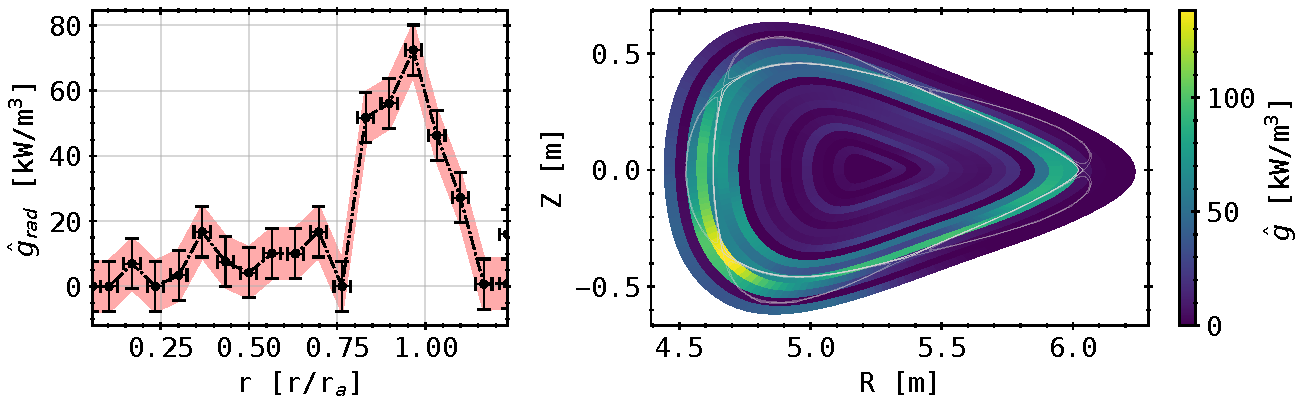
\includegraphics[width=.9\textwidth]{%
                        content/figures/chapter1/mfr2D_example.pdf}\\%
                    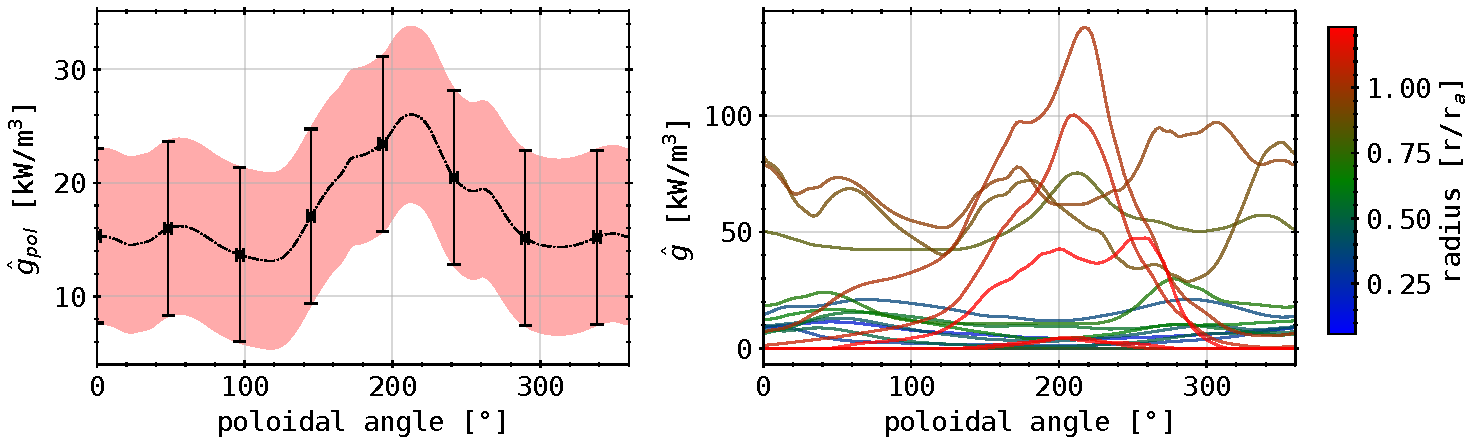
\includegraphics[width=.9\textwidth]{%
                        content/figures/chapter1/mfr2D_poloidal2.pdf}%
                    \caption{%
                        XP20180725.44\\%
                        Example of local radiation distribution profiles at $t=\,$\SI{3.0}{\second}. \textbf{(top-left)}: Poloidally averaged radial radiation profile with absolute vertical and lateral error bars. \textbf{(top-right)}: Two-dimensional radiation distribution, with Poincaré overplot of plasma islands and separatrix. \textbf{(bottom-left)}: Radially averaged poloidal radiation profile with error bars. \textbf{(bottom-right)}: Individual poloidal radiation distribution.}\label{fig:mfr_examples}%
                \end{figure}%
%
                Let us assume an arbitrary inversion that yields a radiation distribution $\mathrel{\hat{g}}\left(\vec{r}\right)$ in the plane of the bolometer cameras. Both radial and poloidal maps of the radiation distribution can be written as:%
%
                \begin{empheq}[box=\fbox]{align}%
                    \mathrel{\hat{g}}\ix{rad}\left(r\right)&=\frac{1}{2\pi}\int_{0}^{2\pi}\mathrel{\hat{g}}\left(r,\vartheta\right)\diff\vartheta\,\,,\label{eq:radial_profile}\\%
                    \mathrel{\hat{g}}\ix{pol}\left(\vartheta\right)&=\frac{1}{f\ix{p}r\ix{a}}\int_{0}^{f\ix{P}r\ix{a}}\mathrel{\hat{g}}\left(r,\vartheta\right)\diff r\,\,.\label{eq:poloidal_profile}%
                \end{empheq}%
%
                \autoref{fig:mfr_examples} shows an example for a two-dimensional radiation distribution and its poloidal and radial integrals in accordance to \cref{eq:radial_profile} and following. The map is based on geometric arguments and the grid discussed in the previous section, especially \cref{eq:emissivity}. Radiation has been reconstructed mainly in the shape of a three to five cell wide ring along the separatrix. The X-point on the lower inboard side however has a maximum that is approximately twofold the average intensity of the radiation ring. Consequently, assuming equal drop-off lengths around the plasma the ring is widened on the inboard side. The radial profile in $\mathrel{\hat{g}}\ix{rad}$ indicates that the radiation is mainly located inside the last closed flux surface, where the intensity increases sharply towards the maximum at $0.95r\ix{a}$. Presented error bars are, on one hand, derived from the mathematical penalty of the inversion algorithm, i.e. the absolute error in emissivity as noted by $\chi$ in \cref{eq:tikhonov_algo}. On the other hand, the error in resolution of the resulting profile is given by half of the width or height of the cells. Plots of individual radial position in the bottom left of \cref{fig:mfr_examples} accentuate asymmetries that are functions of the poloidal angle. The distinct radiation peak is found here between $0.9-1.1r\ix{a}$ at the lower inboard X-point around $230-240^{\circ}$. The average poloidal profile is similarly shaped and supports the previous observations, however at a much lower intensity. This is due to the contribution of the mostly dark areas of the reconstructed image where no emission has been reconstructed by the algorithm.\\%
                The application of an inverse reconstruction algorithm that is tailored towards the problem posed by the previously introduced bolometry system is considered to be best practice in order to assess the local radiation distribution. This however requires a number of assumptions about and \textit{a priori} knowledge of the mathematical procedure and its behaviour, as well as the physics that govern the measurements. A mathematical tool like the \textit{Tikhonov regularisation} with the \textit{Fisher\footnote[1]{Sir Ronald Aylmer Fisher~Feb. 17, 1890 \textdagger~July 29, 1962} information} as a constraint or regulator is of great value towards the understanding of plasma radiation and the underlying impurities. The latter will be characterised in much more detail and an example algorithm outlined in \cref{chap:inversions}.\\%
                \newline%
                After having introduced local and global radiation power measurements from the bolometer one can take the next step and use this knowledge for plasma performance characterisation. The next section will discuss the power balance involving the global power estimation derived in the previous section with \cref{eq:prad_total}.%
%
        \subsection{Power Balance}\label{subsec:power_balance}%
%
            % Power balance.%
            Addressing the power balance, and thereby the underlying conservation of energy, of input heating and external losses, i.e. perpendicular transport across magnetic field lines or radiation, is a critical tool for characterising plasmas in magnetically confined fusion devices. Furthermore, it is crucial for the desirability of magnetic fusion and therefore the success of a potential plasma fusion power reactor\cite{Freidberg2007}. It is important to have an understanding of the physical processes that are connected to the heating and power exhaust, which vice versa can profit from thorough experimental investigations on the plasma power balance. For example, the power loss through impurity radiation is, in addition to being practically unavoidable especially in large scale fusion devices, mandatory in a reactor to reduce the heat flux densities to the targets by dissipation of power in the plasma volume. This radiation, plasma parameters like density and temperature, and the resulting transport are strongly and non-linearly coupled\cite{Hirsch2008}.\\%
            A simple approach to the (global) power balance is the zero-dimensional (0-D) treatment of the conservation of energy. This 0-D model is derived from a full set of three-dimensional fluid equations by making a number of assumptions. Let a pure plasma with $n\ix{e}\approx n\ix{I}=n$ the particle number densities of electrons and ions and $n_{Z}\ll n$ of impurity species $Z$. Similarly, the particle temperatures are $T\ix{e}=T\ix{I}=T$. The plasma is assumed to be fully ionized and in thermodynamic equilibrium. Therefore, the internal energy density $U_{j}$ and particle pressure $p_{j}$ of species $j$ are%
%
            \begin{align}%
                U_{j}=\frac{3}{2}n_{j}T_{j}=\frac{3}{2}p_{j}\,\,\,,\qquad%
                p_{j}=n_{j}T_{j}\,\,.\nonumber%
            \end{align}%
%
            Deriving from the conservation law for energy in fluid dynamics and using the (fluid) velocity $\vec{u}$ one yields the conservation of energy for a zero-dimensional ansatz as\cite{Freidberg2007}:%
%
            \begin{align}%
                \frac{3}{2}\frac{\partial p}{\partial t}+\frac{3}{2}\left(\nabla\cdot p\right)\vec{u}+p\nabla\cdot\vec{u}+\nabla\cdot\vec{q}=s\label{eq:0d_conserve}\,\,.%
            \end{align}%
%
            The right-hand side of \cref{eq:0d_conserve} combines energy sources and sinks in $s$. The first term on the left-hand side describes the energy density variation. A net flux of plasma energy is accredited for in the second term. The third term accounts for changes in energy density under plasma expansion or shrinkage. Finally, the fourth term on the left denotes energy losses through diffusive processes as an energy density current $\vec{q}$.\\%
            At a magnetically confined plasma fusion device the sources and sinks term can be written as\cite{Bozhenkov2016}:%
%
            \begin{align}%
                s=s\ix{H}-s\ix{rad}\,\,.\nonumber%
            \end{align}%
%
            Therein noted energy density input and losses are: $s\ix{H}$ the gain from the input heating and $s\ix{rad}$ the dissipation via plasma radiation.\\%
            Integrating \cref{eq:0d_conserve} over the volume of the plasma yields the simplified null-dimensional global energy balance.%
%
            \begin{align}%
                0&=\frac{1}{V\ix{P}}\int_{V\ix{p}}\left(\frac{3}{2}\left(\frac{\partial p}{\partial t}+\left(\nabla\cdot p\right)\vec{v}\right)+p\nabla\cdot\vec{v}+\nabla\cdot\vec{q}-S\right)\diff\vec{r}\nonumber\\%
                &=-S\ix{H}+S\ix{rad}+S\ix{div}+\frac{1}{V\ix{P}}\int_{V\ix{p}}\left(\frac{3}{2}\left(\frac{\partial p}{\partial t}\right)+p\nabla\cdot\vec{v}+\nabla\cdot\vec{q}\right)\diff\vec{r}\nonumber\\%
                0&=S\ix{H}-S\ix{rad}-S\ix{div}-\frac{\diff W}{\diff t}=S\ix{bal}\label{eq:energy_balance}%
            \end{align}%
%
            In \cref{eq:energy_balance} the volume integral over the net plasma energy flux $3/2\left(\nabla\cdot p\right)\vec{u}$ was accounted for as the convective energy loss to a target $S\ix{div}$. The plasma stored energy is $W$. Experimentally there are, as of now, two possibilities of assessing this number: estimating the total kinetic energy $W\ix{kin}$ using density and temperature profiles or measuring the diamagnetic energy $W\ix{dia}$ with a separate diagnostic.
%
            \begin{align}%
                W\approx W\ix{kin}=\frac{3}{2}\int_{V\ix{P}}\sum_{j}n_{j}T_{j}\frac{\diff V}{\diff r}\diff r\nonumber%
            \end{align}%
%
            Using the kinetic energy as an estimator, although while being analytical, has some drawbacks: derivation of $\diff V/\diff r$ is based on magnetic equilibria, the working gas ion density $n\ix{i}$ is assumed to be equal to $n\ix{e}$ and the contribution of plasma impurities is difficult to address experimentally. Neglecting impurities in $W\ix{kin}$ shows larger values of around 25\%, which again varies with species and density of said impurity, when comparing to the diamagnetic energy\cite{Bozhenkov2016}. Furthermore, electron density and temperature profiles from the \textit{Thomson scattering} diagnostic that have been provided during the previous experimental campaign were very sensitive to inconsistencies in both calibration and laser adjustment\cite{Bozhenkov2017,Pasch2016}. Multiple diamagnetic loops at various locations of W7-X measure magnetic flux changes of the plasma. Those changes are directly related to the plasma stored energy. Thus,the diamagnetic energy, given an adequate model for compensating external magnetic flux contributions, has been consistently and accurately provided by a dedicated diagnostic\cite{Rahbarnia2018}.\\%
            The total time derivative of the energy balance in \cref{eq:energy_balance} yields the power balance of the plasma, with $P\ix{H}=P\ix{ECRH}$ the input microwave electron cyclotron heating:%
%
            \begin{empheq}[box=\fbox]{align}%
                0=\frac{\diff}{\diff t}S\ix{bal}\overset{!}{=}P\ix{bal}=P\ix{ECRH}-P\ix{rad}-P\ix{div}-\frac{\diff W}{\diff t}\label{eq:power_balance}%
            \end{empheq}%
%
            \autoref{eq:power_balance} \textit{de facto} sets the global power balance to zero. However, in practice, when characterising $P\ix{bal}$ using experimentally measured values for the contributing sources and losses, each one introduces errors through simplifications in their respective models and measurement techniques.\\%
            The radiative power loss $P\ix{rad}$ is based on an approximation for the irradiating plasma volume and geometric model for the lines of sight. Additionally, \cref{eq:prad_total} assumes toroidal symmetry of the plasma radiation, while Zhang~et al. have previously found that this is not necessarily the case. Analysis of bolometry data from past experimental campaigns, based on comparisons with other diagnostics involved in the power balance in \cref{eq:power_balance}, indicate a 5\% error for the proxy of the global $P\ix{rad}$ from \cref{eq:prad_total} derived in \cref{subsec:global}. Recently it was discussed that there might a previously neglected contribution of the vessel heat load through plasma radiation from the main chamber. This error is expected to be as large as 25\% of $P\ix{rad}$ in certain scenarios. In addition, the value of input microwave heating power $P\ix{ECRH}$ is noted to have an intrinsic error of 10\%\cite{Marsen2016}. Finally, the divertor target power load $P\ix{div}$ has to be measured. A thermography system consisting of ten infrared cameras, observing all divertor units measure the surface temperature and provide the total power load\cite{Gao2019}. Discrepancies in the measurement of the total target power load occur due to errors in the infrared measurement and its mapping to the individual divertor elements, as well as toroidal asymmetries and errors in the heat transport analysis code THEODOR\footnote[1]{THEODOR: thermal energy onto divertor}. Peak heat loads are found to have an intrinsic error of up to 10\%\cite{Gao2019}.\\%
%
            \begin{figure}[t]%
                \centering%
                \includegraphics[width=\textwidth]{%
                    content/figures/chapter1/%
                    power_balance_example_20180808_004.pdf}%
                \caption{%
                    XP20180808.4\\%
                    Example for power balance as in \cref{eq:power_balance}. \textbf{(top-left)}: Microwave power and divertor target heat loads, including individual elements \textbf{(top-right)}: Radiative power loss as measured by the bolometer cameras \textbf{(bottom-left)}: Plasma stored energy measured by diamagnetic loops and its time derivative \textbf{(bottom-right)}: Individual power balance for both bolometer cameras (blue, red) and a general result from the mean with error bar (grey).}\label{fig:powerbal_0808.004}%
            \end{figure}%
%
            An example for the power balance derived in \cref{eq:power_balance} and the respective quantities involved can be seen in \cref{fig:powerbal_0808.004}. The ECRH delivers, after an initial, slightly decreasing stage of \SI{1.3}{\mega\watt} within the first \SI{0.8}{\second} of the plasma discharge, a constant \SI{0.55}{\mega\watt} of microwave power for the duration of \SI{28}{\second}. The resulting individual divertor target heat loads are below \SI{100}{\kilo\joule} per module and within the previously discussed error bar of the thermography diagnostic, indicating a toroidally symmetric heat load distribution. The total, integrated target load varies across the experiment duration, but remains below \SI{0.5}{\mega\watt} with a gradual increase from $\approx\SI{0.2}{\mega\watt}$ and two drops around \SI{1.75}{\second} and \SI{8.5}{\second}. After shut-off of the heating power, the remaining heat load drops below \SI{250}{\kilo\watt}, but immediately increases again to about \SI{300}{\kilo\watt}. Bolometer measurements and calculations of the global radiative power loss with \cref{eq:prad_total} present a slowly increasing radiation level from \SI{0.15}{\mega\watt} after the initial heating stage to \SI{0.25}{\mega\watt} at the termination of ECRH. Within the first \SI{0.5}{\second}, $P\ix{rad}$ rises to \SI{0.25}{\mega\watt} drops below \SI{0.2}{\mega\watt} again. After microwave heating shut-off, the radiation power peaks with \SI{0.55}{\mega\watt} due to irradiating the remaining plasma energy and recombinations, before sharply decreasing to zero. The diamagnetic energy $W\ix{dia}$ quickly peaks at \SI{220}{\mega\joule} within the first \SI{0.5}{\second}, from which a small drop and increase are followed by a gradual decline with small perturbations to \SI{180}{\kilo\joule} at the end of the discharge. The resulting time derivative $\diff W\ix{dia}/\diff t$ rises to \SI{0.6}{\mega\watt}, as $W\ix{dia}$ goes towards its maximum, and turns over for the enclosed small drop. Over the duration of the experiment, $\diff W\ix{dia}/\diff t$ drifts around zero, although the plasma energy clearly presents a declining slope. At ECRH termination this energy is exhausted from the plasma and its time derivative indicates negative $\SI{0.45}{\mega\watt}$.\\%
            The resulting global power balance is generally satisfied within the given error bar, i.e. $P\ix{bal}\approx 0$. However, there still persist non-negligible discrepancies in the power balance that are not accounted for in the previously discussed plasma properties. For example, in the beginning of the experiment,ana excess of heating power is indicated, as well as the radiation peak after shut-off leads to a large negative balance. Also, one of the drops in target heat load around \SI{8.5}{\second} can not be explained by this model.\\%
%
            \begin{figure}[t]%
                \centering%
                \includegraphics[width=\textwidth]{%
                    content/figures/chapter1/%
                    power_balance_example_20180725_044.pdf}%
                \caption{%
                    XP20180725.44\\%
                    Example discharge as previously exhibited. \textbf{(top-left)}: ECRH power and divertor target heat loads \textbf{(top-right)}: $P\ix{rad}$ as measured by the bolometer cameras \textbf{(bottom-left)}: Plasma stored energy measured in $W\ix{dia}$ and its time derivative \textbf{(bottom-right)}: Power balance for both bolometer cameras (blue, red) and their mean.}\label{fig:powerbal_0725.044}%
            \end{figure}%
%
            Further exemplifying this issue are the results shown in \autoref{fig:powerbal_0725.044}. This is the same experiment as previously discussed in the examples shown in \cref{subsec:local} and \cref{fig:chord_examples} and \cref{fig:mfr_examples}. The heating power is delivering a constant \SI{1}{\mega\watt} for \SI{12.5}{\second}. The displayed individual heat loads are well below \SI{200}{\kilo\watt}. The divertor heat rises with non-negligible retardation to the engagement of the ECRH and only slowly decreases after its shut-off. Following a peak heat load of \SI{0.6}{\mega\watt} around \SI{0.1}{\second}, $P\ix{div}$ decreases with a rate similar to the increase of $P\ix{rad}$. The remaining heat load drifts between \SIrange{0.2}{0.3}{\mega\watt}. Bolometric measurements of this discharge indicate a rapid increase of radiation from the engagement of the heating to \SI{3.0}{\second}, where previously a significant shrinkage of the plasma was discussed in \cref{subsec:local} with \cref{fig:chord_examples}. In the following \SI{2}{\second} the radiation power is substantially larger than the input heating. This is a strong indication for errors in the volumetric estimation of \cref{eq:prad_total}, especially considering the results of $P\ix{bal}$ and $\diff W\ix{dia}/\diff t$ for those times. From there on, $P\ix{rad}$ very slowly decreases until plasma termination, about \SI{0.5}{\second} after heating shut-off, where it still measures about \SI{1}{\mega\watt}. The diamagnetic energy sharply rises to its maximum at \SI{0.5}{\second} of \SI{175}{\kilo\joule} and then drops to \SI{100}{\kilo\joule}, before it quickly increases again to \SI{160}{\kilo\joule} towards the plasma collapse at \SI{3.1}{\second}. After that the remaining plasma stored energy almost zeros and is as small as \SI{50}{\kilo\joule}.\\%
            The resulting power balance shows large deviations from zero, indicating inconsistencies between the physics of the presented plasma and the model of the power balance \cref{eq:power_balance}. At the start of the discharge $P\ix{bal}$ in \cref{fig:powerbal_0725.044} appears to be a poor measure for energy conservation. After ECRH start-up $P\ix{bal}$ quickly turns negative and immediately inverts due to the simultaneous increase of $P\ix{rad}$, $\diff W\ix{dia}/\diff t$ and the reversal of the latter. Before \SI{3.0}{\second} the power balance indicates an excess of heating power that is not accounted for in any of the above. Towards the maximum of radiation power at \SI{3.1}{\second}, $P\ix{bal}$ turns negative again, while $\diff W\ix{dia}/\diff t$ is also negative, indicating that $P\ix{rad}$ greatly overestimates the true radiative power loss in this case. The balance then drifts towards zero until the termination of ECRH, were radiation from the collapsing plasma lead to a negative pedestal that fades with its extinction.\\%
            The presented global plasma power balances exemplify the applicability of the model discussed in \cref{eq:power_balance}. One expects scenarios with fast plasma transitions, i.e. strong perturbations and variations in profiles or plasma properties, to be not very well described by this approach. Though it is assumed that steady state conditions are represented much better by this model.\\%
            \,\newline%
%